 \documentclass[paper=a4, DIV=14, BCOR=15mm, twoside=on, onecolumn=on, open = right, titlepage =on, parskip =half, headsepline = on, footsepline = on, chapterprefix = on, appendixprefix = off, fontsize = 12pt, numbers = noenddot, abstract = on]{scrbook}
\usepackage[utf8]{inputenc}
\usepackage[german]{babel}
\usepackage{amsmath}
\usepackage{amsthm}
\usepackage{amsfonts}
\usepackage{amssymb}
\usepackage{makeidx}
\usepackage{graphicx}
\usepackage{tikz}
\usepackage{wrapfig}
\usepackage{geometry}
\usepackage{parallel}
\usepackage{todonotes}
 \usepackage{mathptmx}
 \usepackage{pdfsync}
 \usepackage{url}
 \usepackage{float}
 \usepackage{hyperref}

 %\usepackage[scaled=.90]{helvet}
 \usepackage[T1]{fontenc} 
%\newcommand{\changefont}[3]{ \fontfamily{#1} \fontseries{#2} \fontshape{#3} \selectfont}
%\changefont{cmr}{m}{n} %ppl for Palatino, ptm for Times New Roman
\setkomafont{title}{\rmfamily \bfseries}
\setkomafont{chapterentry}{\rmfamily \bfseries}
\usepackage{cutwin}
\usepackage[raggedleft]{titlesec}
\titlelabel{\thetitle.\quad}
\titleformat*{\chapter}{\scshape\bfseries\large}
\titleformat*{\section}{\bfseries\large}
\titleformat*{\subsection}{\bfseries \normalsize}
\titleformat*{\subsubsection}{\bfseries \normalsize}

\DeclareMathOperator{\GL}{GL} % einige Macro, siehe am Ende Abschn. 2
\newcommand{\N}{\mathbb{N}}
\newcommand{\Z}{\mathbb{Z}}
\newcommand{\Q}{\mathbb{Q}}
\newcommand{\R}{\mathbb{R}}
\newcommand{\C}{\mathbb{C}}
\newcommand{\cP}{{\mathcal P}} 








\usepackage{blindtext}
\usepackage{todonotes}


\usepackage[german]{babel}
\usepackage{setspace}
%\usepackage[linkbordercolor={1 1 1}]{hyperref}\urlstyle{rm}

\begin{document}
\newpage
\thispagestyle{plain}

%\pagenumbering{Roman}


\begin{titlepage}


\begin{figure}[htbp]
		\begin{minipage}[b]{25mm}
			
\includegraphics[width=25mm,clip]{images/logo_uhh}
		\end{minipage}
		\begin{minipage}[b]{2mm}
			
\includegraphics[width=1mm,height=25mm]{images/greypixel}
		\end{minipage}
		\begin{minipage}[b]{12.5cm}
			{   
				\vspace{2mm}
				{\Large Universität Hamburg } \\
				Fakultät für Mathematik,\\
				Informatik und Naturwissenschaften \\
				Department Informatik \\
			}
		\end{minipage}
	\end{figure}


\begin{center} 
\vspace{0.5cm} 
\begin{tabular}{c}
% \vspace{0.5cm}\\
\Large \textsc{Entwicklung einer Java Simulationsumgebung}\\
 \\
\Large \textsc{für Lego Mindstorms NXT Roboter}\\
\\
\\
\small Masterarbeit im Fach Informatik zur Erlangung des akademischen Grades\\
\\
\normalsize \textbf{Master of Education}\\
\\
\small im Studiengang Lehramt an Gymnasien M.Ed.\\
\\
\\
\large \textbf{Pamina Maria Berg}\\
\small \emph{Matr.Nr. 6087438}\\
\\
\normalsize Hamburg, den \today
\end{tabular}
\par 
\end{center}
\par
\vspace*{3cm}
\begin{tabular}{l}
\emph{Erstgutachter}\\
Dr.\, Guido Gryczan\\
\emph{Zweitgutachter}\\
Jun.-Prof.\, Dr. Maria Knobelsdorf\\
\emph{Betreuer}\\
Till Aust\\
Fredrik Winkler\\
\end{tabular}

\end{titlepage}


\thispagestyle{empty}
\cleardoublepage
\newpage
\listoffigures
\newpage
\tableofcontents
\thispagestyle{empty}
\cleardoublepage
\newpage
%\pagenumbering{arabic}
\par \singlespacing
\chapter{Einleitung}
\onehalfspacing
"`Informatik in der Schule"' ist ein bildungspolitisch umfassend diskutiertes Thema der letzten Jahre. Eine zentrale Rolle nimmt dabei die Frage ein, ob es sinnvoll sei, ein Unterrichtsfach "`Programmieren"' ab der Grundschule einzuführen, oder ob es reicht, dass die Schülerinnen und Schüler dazu ausgebildet werden, einen Computer bedienen zu können. Dabei stehen sich die Grundgedanken der beiden Extreme, nämlich die Schülerinnen und Schüler als kompetente Computer-Nutzer mit einem Verständnis der logischen Strukturen hinter der Benutzeroberfläche auf der einen und das Heranziehen einer Generation von Schülerinnen und Schülern, die auf die Verwendung der gängigen Office-Anwendungen geschult wurde, auf der anderen Seite, gegenüber.

In der gymnasialen Oberstufe ist das Erlernen einer Programmiersprache derzeit schon vorgesehen. Doch auch ab der fünften Klasse kann bereits mit dem Erlernen von objektorientierten Programmierparadigmen begonnen werden. Eine wertvolle Ergänzung des klassischen Unterrichts hat sich in den letzten Jahren aus der Entwicklung der Ganztagsschulprogramme herauskristallisiert -- im Nachmittagsbereich wurden nun neben sportlichen und musisch-künstlerischen Angeboten sowie klassischer Nachhilfe Roboter-AGs gegründet, in denen Schülerinnen und Schüler an die Technik von verschiedensten programmierbaren Robotern herangeführt werden.\\
Auf spielerische Art und Weise sollen Schülerinnen und Schüler (im Folgenden SuS abgekürzt) mit einfachen Konstrukten der objektorientierten Programmierung umzugehen lernen. Der Grundgedanke hinter diesem Konzept reicht bis in die Siebzigerjahre des letzten Jahrhunderts: Der Mathematiker, Informatiker und Psychologe Seymour Papert hat schon damals herausgefunden, dass das Ziel, Kinder zum Programmieren zu bringen, mithilfe einer spielerischen Herangehensweise erreicht werden könnte. Hierdurch entstand das bis heute bekannte Konzept der \emph{Turtle} (vgl. \cite[S.365]{nievergelt:99}).\\
Heutzutage wird der spielerische Aspekt beim Programmieren im Zusammenhang mit \textsc{LEGO Mindstorms} Robotern zum einen mit Drag-and-Drop Softwareangeboten wie das standardmäßig mit ausgelieferte \emph{NXT Mindstorms Tool} (s.  \textbf{\ref{sec:LMNXT}}), oder auch \emph{Enchanting} (s. \textbf{\ref{sec:enchanting}}) realisiert. Zum anderen bietet sich ab der Mittelstufe (Klasse 7 -- 10) die Arbeit mit BlueJ zur Erstellung erster selbstgeschriebener Programme an. Hierzu kann eine BlueJ Extension genutzt werden, die mit der Java Virtual Machine \emph{leJOS NXJ} für NXT Roboter (s. \textbf{\ref{sec:lejos}}) arbeitet.

Immer wieder stoßen Lehrkräfte in den Schulen auf Hardwareprobleme jeglicher Art, wie zum Beispiel eine unzureichende Anzahl an Robotern im Unterricht oder auch fehlende Firmwareupdates oder defekte Sensoren.\\
Auch das Zusammen- und wieder Auseinanderbauen der Roboter ist ein Aufwand, der für den alltäglichen Unterricht nicht geeignet ist. Um kleine Aufgaben -- wie zum Beispiel das Fahren einer Kurve oder das Anhalten auf einem bestimmten Punkt -- mit Java zu lösen, muss bisher immer erst der Roboter gestartet, der Code in BlueJ verfasst und auf den Roboter übertragen werden. Schließlich muss der Roboter noch zu einem geeigeneten Parcours gebracht werden, um die Lösung testen zu können.

Um diese Probleme zu umgehen und den Einstieg in die objektorientierte Programmierung über die Benutzung von \textsc{LEGO Mindstorms} Robotern zu optimieren, soll im Rahmen dieser Masterarbeit der Protoyp einer Simulationsumgebung für die Arbeit mit \textsc{LEGO Mindstorms} NXT Roboter entwickelt werden.
\newpage
\par\singlespacing
\chapter{Ausgangssituation}

\par\singlespacing
\section{Das LEGO Mindstorms NXT System}
\onehalfspacing
Die ersten computergesteuerten \textsc{LEGO} Produkte wurden bereits 1986 veröffentlicht. In einer Zusammenarbeit von \textsc{LEGO} Education und dem Massachussettes Institute of Technology (MIT) wurde \textsc{LEGO TC LOGO} entwickelt. Dies war eine spezielle Abwandlung der Programmiersprache LOGO, mit der zusammengesetzte \textsc{LEGO}-Modelle gesteuert werden konnten (vgl. \cite{rolling:14}).\\
Die Entwicklung eines programmierbaren \textsc{LEGO}-Steins begann 1988 und erreichte ihren Höhepunkt mit der Vorstellung des ersten Mindstorms Systems im Januar 1998, bei der der \textsc{LEGO Mindstorms RCX Intelligent Brick} -- ein Microcomputer und somit das Kernstück des RCX-Systems -- und das \emph{Robotics Invention System} im Museum of Modern Art in London vorgestellt wurden.\\
Bereits zwei Monate nach Verkaufsstart wurde die FIRST LEGO League (FLL) gegründet -- eine Zusammenarbeit zwischen \textsc{LEGO} und FIRST (For Inspiration and Recognition of Science and Technology), die den Grundstein für die heute noch bestehende Wettbewerbsliga legte (vgl. \cite{rolling:14}).\\
Die Vorstellung und der Verkaufsstart der Nachfolge-Roboter des RCX-Systems, den \textsc{LEGO Mindstorms} NXT Robotern, fand im August 2006 statt. Diese damals neu entwickelten Roboter sind dank eines Updates in 2009 fast zehn Jahre später noch in den Schulen und Universitäten zu finden. Im April 2005 fand die erste FLL Weltmeisterschaft in Atlanta, Georgia, statt und bis heute bieten die Weltmeisterschaften einen Anlaufpunkt für Jugendliche auf der ganzen Welt, die ihr Können und ihre Roboter auf die Probe stellen wollen (s. \cite{lego}).

\par \singlespacing
\subsection{Hardware}
\onehalfspacing
Zentraler Bestandteil der \textsc{LEGO Mindstorms} NXT Roboter ist der sogenannte NXT-Stein. Dieser besteht aus einem 32 Bit RAM-Prozessor und einem 8 Bit Co-Prozessor. Der Hauptprozessor ist für die Ausführung des Hauptprogramms zuständig, während sich der Co-Prozessor um die Auswertung etwaiger Sensordaten kümmert, die dann an den Hauptprozessor weitergeleitet werden. Für die Kommunikation mit dem NXT-Stein stehen zwei Komponenten zur Verfügung. Zum einen eine Kabelverbindung mit einer USB 2.0 Schnittstelle, zum anderen bietet der NXT-Stein -- wie schon der Vorgänger RCX -- die Möglichkeit einer Kommunikation über Bluetooth an. Das Softwaremenü wird auf dem 100 x 64 Pixel großen LCD-Bildschirm angezeigt und kann über die vier Kontrolltasten auf der Oberseite des NXT-Steins bedient werden. Für eine ausreichende Stromversorgung wird entweder mittels Batterien oder eines Akkus gesorgt (vgl. \cite[S.42]{berns:10}).\\
Der NXT-Stein verfügt standardmäßig über drei Motoranschlüsse (\emph{Motorports}) und vier Sensoranschlüsse (\emph{Sensorports}), die jeweils mit Buchstaben (\emph{A, B, C} bei den Motoren) bzw. Nummern (\emph{1, 2, 3, 4} als Sensoranschlüsse) bezeichnet sind(vgl.  \cite[S.43]{berns:10}). An zwei der drei verfügbaren Motorports ist jeweils ein Elektromotor angeschlossen. In diese Motoren sind Rotationssensoren und Regler eingebaut, die dafür sorgen, dass sowohl die Drehgeschwindigkeit als auch die Umdrehungszahl mithilfe des Programmcodes kontrolliert werden kann (vgl. \cite[S.45--47]{berns:10}).\\
Für die NXT Roboter sind eine Vielzahl von Sensoren verfügbar, damit die SuS ihren Roboter sein Umfeld erkunden lassen können. Eine umfassende Übersicht der einzelnen Sensoren und deren spezifischen Funktionsweisen geben \textsc{Berns} und \textsc{Schmidt} (s. \cite[Kapitel 4.2]{berns:10}). 

\par \singlespacing
 \section{Die Arbeit mit LEGO-Robotern im Unterricht}
\onehalfspacing
Die Robotik als Teilgebiet der Informatik in der Schule gewinnt zunehmend an Bedeutung. Nicht nur die Programmierung steht im Vordergrund, sondern auch die Kompetenz, Probleme unter bestimmten Aufgabenstellungen zu lösen. \textsc{Berns} und \textsc{Schmidt}, die Verfasser eines der Kernwerke für den Unterricht mit dem \textsc{LEGO Mindstorms} System, schreiben, dass bei der Arbeit mit Robotern im Unterricht "`durch eine konkrete Aufgabenstellung, das problemspezifische Konstruieren und Programmieren eines Roboters sowie durch das letztendliche Testen der gesamte Ablauf eines Problemlösungsprozesses kennen gelernt"' \cite[S.2]{berns:10} wird.

In diesem Zusammenhang kann auch, wie von \textsc{Wagner} ausführlich begründet, die Kooperationsfähigkeiten der SuS im besonderen Maße gefördert werden. Gründe hierfür bestehen unter anderem in der Vielzahl der Möglichkeiten, ein Problem mit Robotern zu lösen, die alle unterschiedliche gut geeignet sind, und durch die die SuS zur Kommunikation und dem Verständlichmachen ihrer Ideen im Team angeregt werden. Hierbei ist das Augenmerk auch auf die Kontrollinstanz zu legen -- nimmt sonst die Lehrkraft diese Rolle für sich ein, so ist der Roboter bei dieser Art von Unterricht eine neutrale, unbestechliche und jederzeit verfügbare Möglichkeit, die geleistete Arbeit zu bewerten (vgl. \cite[S.6f.]{wagner:05}).

\textsc{Schreiber} fasst in seiner Examensarbeit den Einsatz von \textsc{LEGO Mindstorms} Robotern wie folgt zusammen
\begin{quote}
"`Als herausragende Qualität des Materials LEGO-Mindstorms erwies sich die damit erzielbare \textbf{Motivation}, welche ein hohes Maß an Selbsttätigkeit auch über einen längeren Zeitraum möglich machte. Diese Selbsttätigkeit ist die Form des idealen Lernen im Sinne der Handlungsorientierung und hat sich auch in dem durchgeführten Unterricht bewährt. [...] Die \textbf{Sozialform} der Partnerarbeit erwies sich als weit gehend produktiv, zum einen, weil inhaltlich miteinander beraten werden konnte und wurde [...], zum anderen, weil ein LEGO-Mindstorms-Roboter auch für zwei gleichzeitig tätige Personen genug Handlungsmöglichkeiten bietet"' \cite[S.47f.]{schreiber:04}.
\end{quote}
Ähnlich beschreibt es auch \textsc{Stolt} in seiner Ausarbeitung:
\begin{quote}
"`Ein großer Punkt, der für das Roboterlabor spricht, ist das starke Motivationspotential für die Teilnehmer sich mit Informatikthemenstellungen zu befassen. Die Entwicklung einer eigenen Lösung einer Aufgabe, mit anschliessendem Wettbewerb besitzt trotz – oder vielleicht gerade wegen – der möglichen Komplexität einen sehr großen Unterhaltungswert und stelle eine spannende Herausforderung dar. Pädagogisch ist das Roboterlabor durch seine teamorientierte Arbeitsweise und die Möglichkeit zum explorativen Lernen interessant. Didaktisch steht hier das Erlernen und Erfahren von Programmier- und Designmethoden im Vordergrund"' \cite[S.5f.]{stolt:01}.
\end{quote}

Grundsätzlich ist also zu sagen, dass der Einsatz von Robotern im Unterricht als sowohl didaktisch sinnvoll gesehen wird, also auch die Motivation der SuS in diesem Zusammenhang einen starken Einfluss auf den Lernerfolg und die Selbstständigkeit haben können.\\

Es erfolgt nun zunächst die curriculare Einordnung des Themas Roboter im Unterricht in die Bildungspläne aus Hamburg. Danach werden verschiedene Arbeitsmethoden im Zusammenhang mit dieser Art von Unterricht vorgestellt.

\subsection{Curriculare Einordnung}
Die fachlichen Inhalte, die mithilfe des Einsatzes von Robotern im Unterricht vermittelt werden können, sind sowohl im Bildungsplan der Sekundarstufe I für das Gymnasium (Klasse 7 -- 10) und die Stadtteilschule (Klasse 7 -- 11), als auch im Bildungs- bzw. Rahmenplan für die Gymnasiale Oberstufe, der Sekundarstufe II, verankert. Der folgende Abschnitt gibt eine Übersicht über die verschiedenen Module im Zusammenhang mit den Unterscheidungen zur Schulform und Klassenstufe. 

\subsubsection{Gymnasium Sekundarstufe I (7 -- 10) Informatik Wahlpflicht}
Der Einsatz von Robotern kann auf die Module 2 und 3 des Bildungsplanes für die Sekundarstufe I des Gymnasiums bezogen werden. Hier heißt es\\

 \begin{quote}
Modul 2
\begin{itemize}
\item Abläufe analysieren und umgangssprachlich beschreiben, zu Algorithmen formalisieren und mit einer formalen Sprache implementieren
\item Umgang mit einer einfachen Entwicklungsumgebung
\item Testen, Ergebnisse interpretieren und bewerten
\item Grundlagen der prozeduralen Programmierung: Sequenz, Alternative, Wiederholung, Prozedur bzw. Funktion
\end{itemize}
\vspace*{1cm}
Modul 3 -- Kontext Daten und Prozesse
\begin{itemize}
\item Grundlagen der prozeduralen Programmierung
\item Abläufe formalisieren
\item Algorithmen mit einer formalen Sprache implementieren
\item Testen, Ergebnisse interpretieren und bewerten \qquad \cite{gymsek1:11} 
\end{itemize}
 \end{quote}



\subsubsection{STS Sekundarstufe I (7 --11) Informatik}
Ähnlich ist es im Bildungsplan für die Stadtteilschulen. Hierbei werden allerdings innerhalb der Module verbindliche Inhalte formuliert.

So sind im Modul 2 die Inhalte \emph{Algorithmen} und \emph{prozedurale Programmierung: Sequenz, Alternative, Wiederholung, Funktion} zu finden, die, wie der Bildungsplan vorschlägt, in das Unterrichtsvorhaben \emph{"Wir lassen Roboter arbeiten"} integriert werden können.

Im Modul 3 sollen im zweiten Halbjahr die verbindlichen Inhalte
\begin{itemize}
\item \emph{Grundlagen der prozeduralen Programmierung}
\item \emph{Abläufe formalisieren}
\item \emph{Algorithmen mit einer formalen Sprache implementieren}
\item \emph{Testen, Ergebnisse interpretieren und bewerten}
\end{itemize}
unterrichtet werden \cite{stsmittel:14}. 


\subsubsection{Gymnasiale Oberstufe -- Vorstufe}

In der Vorstufe sollen sich die SuS mit den Inhalten des Moduls \emph{Daten und Prozesse} beschäftigen. Diese beinhalten das Analysieren und umgangssprachliche Bescheiben von Abläufen, das Strukturieren von Daten sowie die Verwendung von Variablen und Parametern, das Formalisieren von Abläufen, die Grundlagen der prozeduralen Programmierung, die Implementation von Algorithmen mit einer formalen Sprache, das Testen, Interpretieren und Bewerten von Ergebnissen \cite{oberstufe:09}. 

\subsubsection{Gymnasiale Oberstufe -- Studienstufe}

In der Studienstufe gibt es den verbindlichen Inhalt \emph{Objektorientierte Modellierung}, der die folgenden Punkte umfasst:\\
\begin{quote}
\begin{itemize}
\item Idee des OO-Konzepts mit Objekten und ihrer Kommunikation, Vererbung und Nutzerbeziehung
\item Erarbeitung der Sprachelemente der verwendeten objektorientierten Programmiersprache, Berücksichtigung von Programmierkonventionen, Nutzen von Bausteinen/Libraries
\item Nutzung einer IDE mit UML-Diagrammen und Quellcode zur schrittweisen Implementierung eines Informatiksystems. \qquad \cite{oberstufe:09}
\end{itemize}
\end{quote}


\subsubsection{Genereller Einsatz von Robotern als Hilfsmittel im Unterricht}
Da laut Bildungsplan die projektorientierte Arbeit in Informatik in der Studienstufe einen bedeutenden Stellenwert hat, bietet es sich natürlich an, eine Projektarbeit zum Thema \emph{Einsatz von Robotern} mit Bezug auf verschiedene Ligen (schulisch und universitär) zu gestalten, bei der als Produkt eine bestimmte Aufgabe mit den Robotern erledigt werden soll.  Diese projektorientierte Arbeit hat den Vorteil, dass sie an einen realen Kontext geknüpft oder in ihn eingebettet werden kann. Wie \textsc{Hubwieser} in seinem Werk \emph{Didaktik der Informatik} verdeutlicht, kann dies einen positiven Einfluss auf die innere Einstellung der SuS gegenüber diesem teilweise recht anspruchsvollen Thema haben.
\begin{quote}
"`Nach den Erfahrungen mit der Umsetzung abstrakter Konzepte [...] im Mathematikunterricht des Gymnasiums scheint eine Vermittlung der naturgemäß abstrakten informatischen Lerninhalte nur dann erfolgversprechend, wenn durch konkrete, anschauliche Problemstellungen eine erhöhte Aufnahmebereitschaft der Schüler geschaffen wird "' \cite[S.68]{hubwieser:07}.
\end{quote}

Die einfachste Methode, um SuS an die problemorientierte Arbeitsweise im Rahmen der Programmierung mit Robotern heranzuführen ist der Einsatz von Fallbeispielen. Hierbei handelt es sich um aus der Realwelt gegriffene Umgebungen, die in unserem Fall mithilfe des Roboters erkundet werden sollen. Ein klassisches Fallbeispiel für den Einstieg wäre die Situation, dass der Roboter vor einem Hindernis steht, um das er herumfahren soll. Hierbei kann man den SuS vorgeben, dass sie z.B. im Viereck um das Hindernis herum navigieren sollen.\\
Ein weitaus komplexerer Beispiele bietet sich im Zusammenhang mit der RoboCup Wettbewerbsliga \emph{Rescue} an, in der ein in einem Labyrinth verstecktes Opfer gerettet werden soll. Hierbei würden sich nun die SuS damit beschäftigen, wie sie durch das Labyrinth navigieren, wie sie Hindernissen ausweichen, und welche bautechnischen Spezifikationen ihr Roboter haben muss, um das Opfer an einen sicheren Ort zu transportieren.

\chapter{Bisher verfügbare Softwarelösungen}
\label{sec:software bisher}
In diesem Kapitel werden nun eine Auswahl von verfügbaren und im Unterricht getesteten Softwarelösungen zur Programmierung der NXT Roboter, sowie einige bereits verfügbare Simulationsumgebungen vorgestellt. 

\section{LEGO Mindstorms NXT}
\label{sec:LMNXT}

Das \textsc{LEGO Mindstorms} NXT-Programm ist eine von der Firma \textsc{LEGO} zur Verfügung gestellte Programmieroberfläche für NXT-Roboter.

\begin{figure}[htbp]
\centering
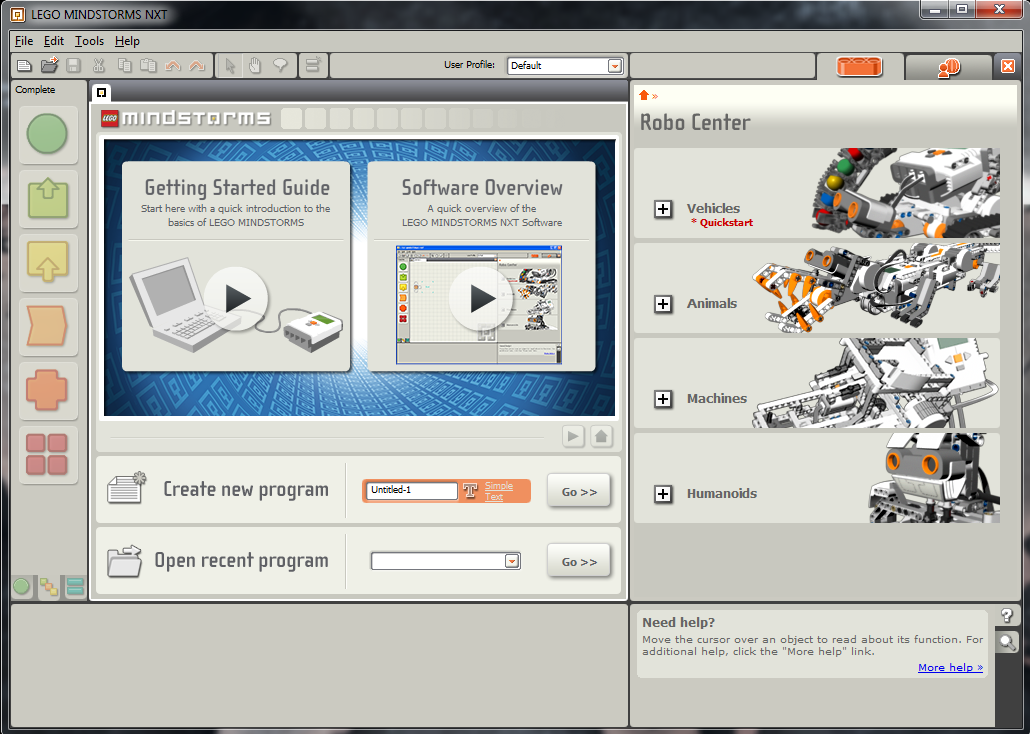
\includegraphics[scale=0.54]{images/Startbildschirm_NXT.png} 
\caption{Der Startbildschirm des \textsc{LEGO Mindstorms} NXT-Programms}
\label{fig:NXT Start}
\end{figure}
Die Abbildung \ref{fig:NXT Start} zeigt den Startbildschirm der Entwicklungsumgebung. Dieser stellt neben zwei Videoanleitungen als Hilfe für Anfänger auch das \emph{Robo Center} zur Verfügung, in dem verschiedene von \textsc{LEGO} vorgeschlagene Roboter-Modelle vorgestellt werden, die mithilfe des Bausatzes des NXT zusammengesetzt werden können.

Sobald eine neue oder bestehende Programmdatei geöffnet wird, können die SuS ihren Roboter programmieren. Hierbei helfen ihnen Blöcke, die unter anderem der Bewegung und Sensorik dienen und dabei einfache Steuerungsmechanismen sowie Elemente der Regelungstechnik zur Verfügung stellen. Zur Programmierung werden Bausteine aus der linken Leiste per Drag-and-Drop auf die karierte Oberfläche gezogen. Es können ineinander geschachtelte Schleifen erstellt werden sowie if-Abfragen mit zwei Fallunterscheidungen. Nahezu beliebig viele Bausteine lassen sich so miteinander kombinieren (Vlg. Abb.\ref{fig:Bsp NXT}).

Der Vorteil an dieser Entwicklungsumgebung besteht darin, dass sie von \textsc{LEGO} zur Verfügung gestellt wurde, und somit alle Funktionen von Haus aus mitbringt, die dem NXT-Baustein technisch zur Verfügung stehen. Zudem muss es keine Veränderungen an der Firmware des NXT-Bausteins geben, was eine Zeitersparnis bei der Vorarbeit der SuS mit sich bringt.

\begin{figure}[htbp]
\centering
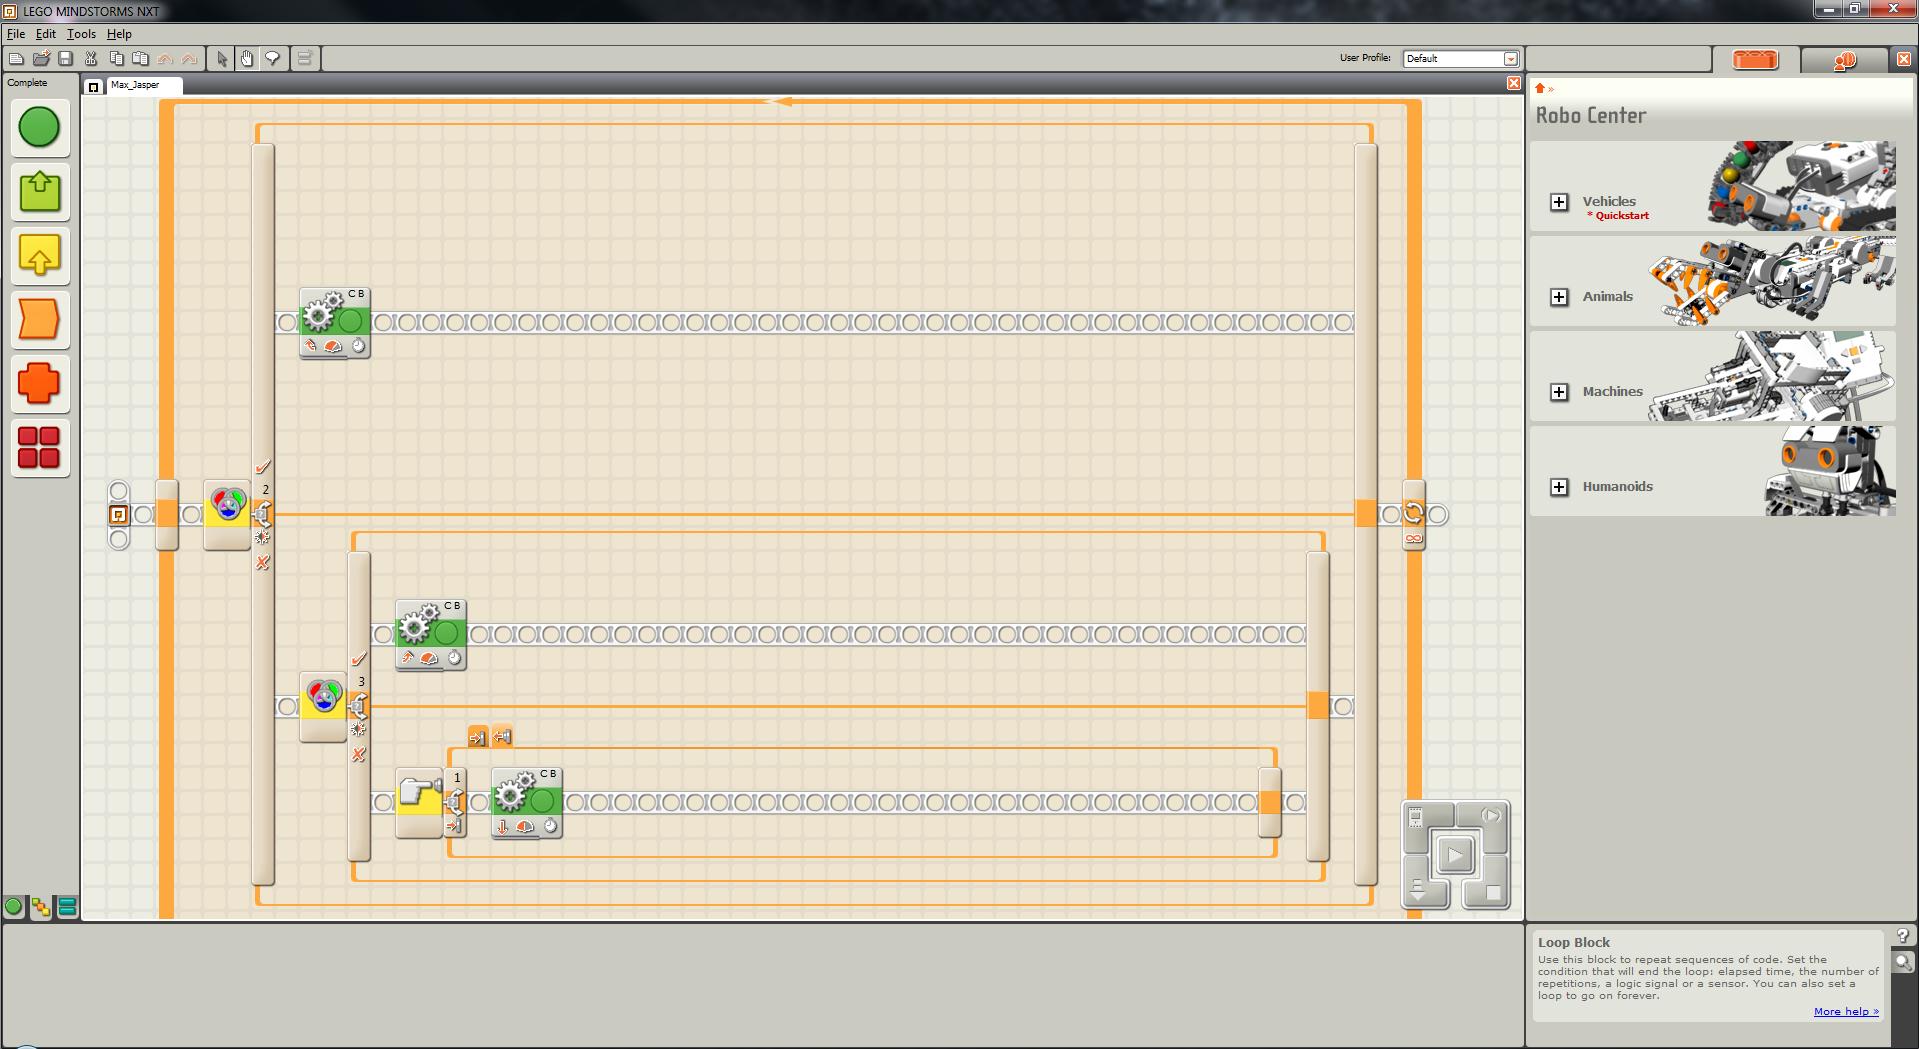
\includegraphics[scale=0.282]{images/Beispielprogramm_NXT.png} 
\caption{Fahren eines Roboters auf einer schwarzen Linie}
\label{fig:Bsp NXT}
\end{figure}

\section{Enchanting}
\label{sec:enchanting}
Enchanting ist eine an das Einsteigertool für Objektorientierte Programmierung \emph{Scratch} anknüpfende Entwicklungsumgebung. Wie das in \textbf{\ref{sec:LMNXT}} beschriebene Programm wird auch hier mithilfe von Drag-and-Drop gearbeitet. Da Enchanting keine von LEGO nativ unterstützte Entwicklungsumgebung für NXT Roboter ist, muss hier eine Änderung an der Firmware vorgenommen werden. Hierbei wird die ausgelieferte Standardfirmware mit leJOS (s. \ref{sec:lejos}) ersetzt. Dies sorgt dafür, dass der NXT nun auf die Programmierung mit Java reagiert.

\begin{figure}[H]
\centering
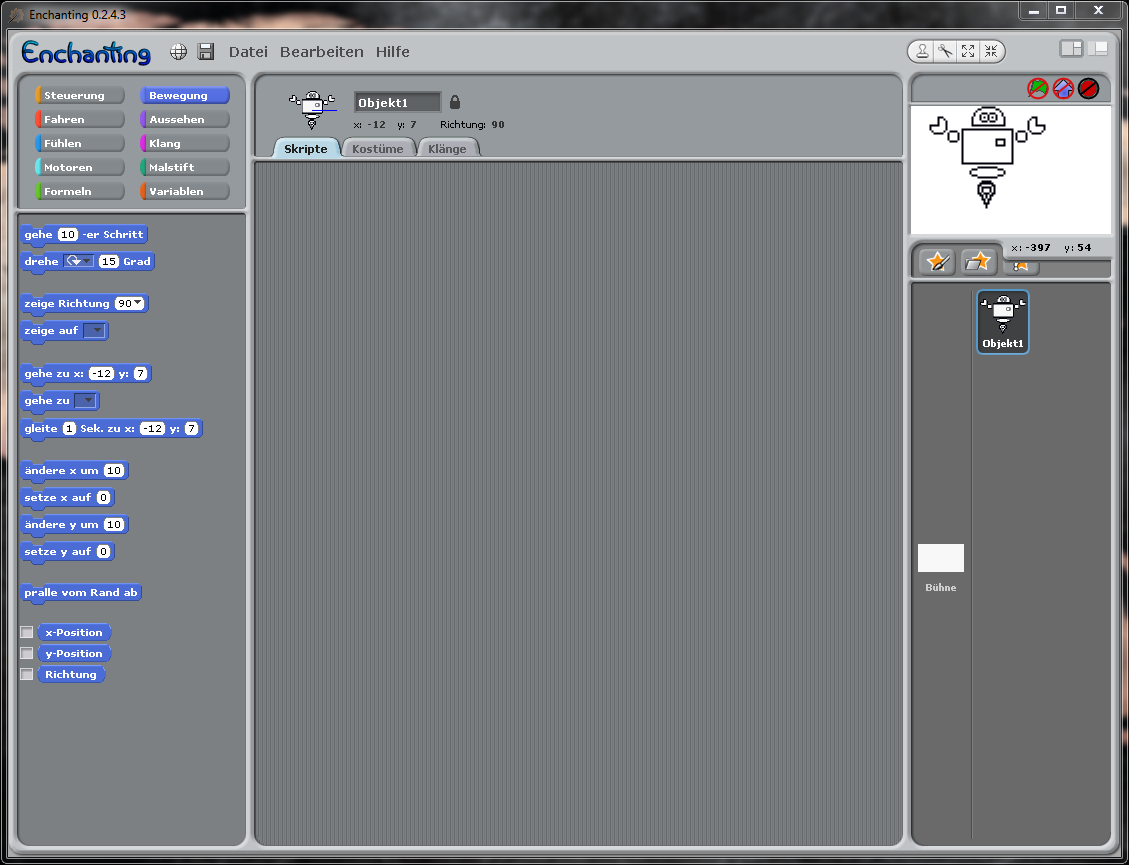
\includegraphics[scale=0.5]{images/Enchanting_Start.png} 
\caption{Der Startbildschirm von Enchanting}
\label{fig:Enchanting Start}
\end{figure}

Wird Enchanting von den SuS geöffnet, erscheint zunächst der Startbildschirm wie in Abb. \ref{fig:Enchanting Start}. Nun kann entweder ein neues Programm erstellt oder ein bestehendes geöffnet werden. Die verschiedenen Programmierelemente werden nach Kategorien in den oberen linken Ecke sortiert aufgeführt. Essentiell dabei sind die Kategorien \emph{Steuerung}, \emph{Fühlen}, \emph{Motoren} und \emph{Formeln}. Die SuS lernen beim Programmieren mit Enchanting, dass sie ihre Motoren und Sensoren zunächst über die verschiedenen Ports referenzieren müssen. Dies geschieht, indem man beispielsweise einen Motor-Block an einen Port setzt und ihm einen aussagekräftigen Namen gibt. Auf diese Weise kann nun -- anders als beim \textsc{LEGO Mindstorms} NXT-Programm -- bei Kontrollstrukturen mithilfe des Namens auf den Motor oder Sensor zugegriffen werden.

In Abbildung \ref{fig:Bsp Enchanting} ist nun ein simples Programm zum Fahren entlang einer schwarzen Linie mithilfe von zwei Lichtsensoren dargestellt. Hierbei ist zu erkennen, dass die Sensoren in den Abfrage-Blöcken mit \texttt{rechts} und \texttt{links}, die Motoren in den türkisfarbenen Elementen mit \texttt{NXT rechts 1} sowie \texttt{NXT links 2} bezeichnet sind. Es kann somit von den SuS direkt gesagt werden, welcher Sensor angesprochen wird, und welcher Motor an welchem Port angeschlossen ist.

\vspace*{2cm}

\begin{figure}[htbp]
\centering
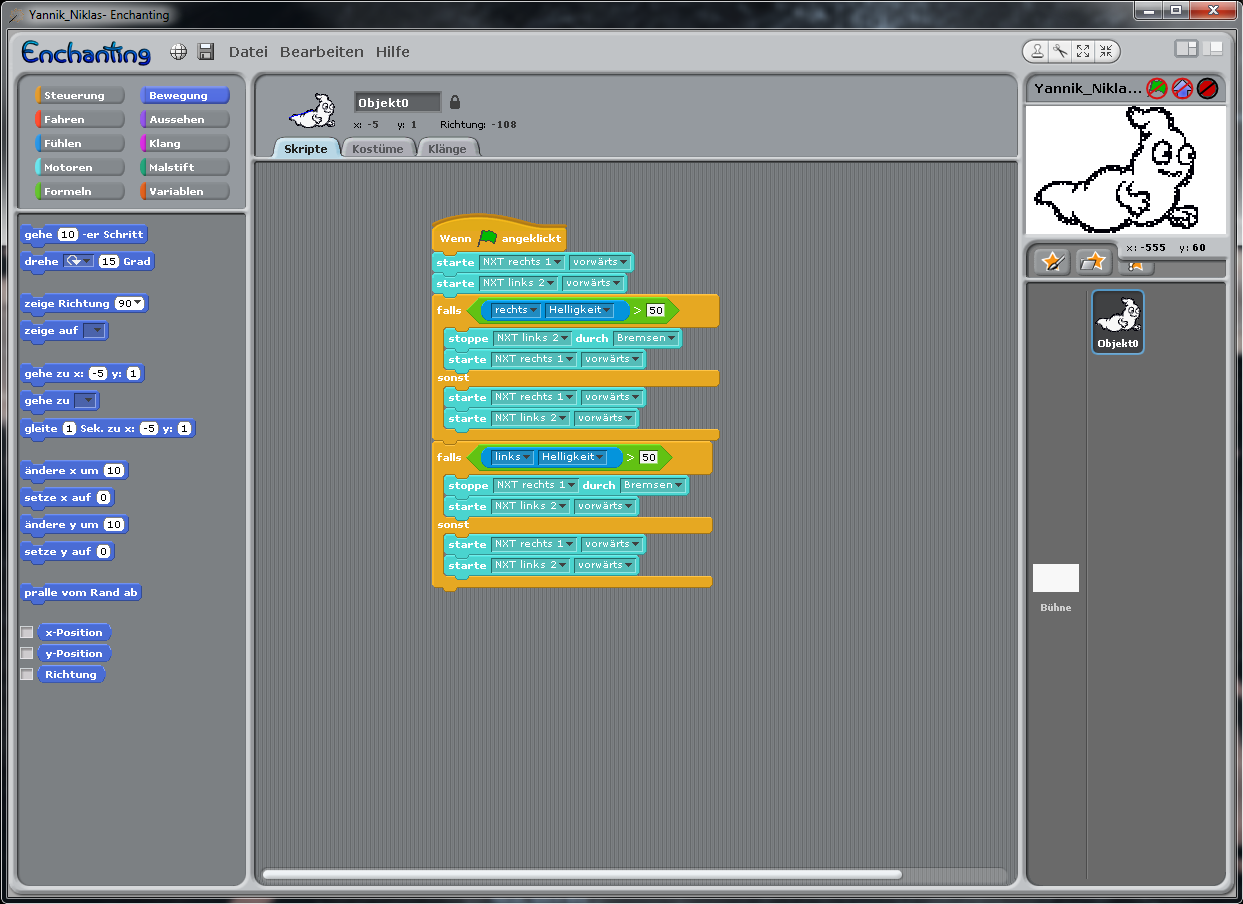
\includegraphics[scale=0.45]{images/Beispielprogramm_Enchanting.png} 
\caption{Beispiel eines Enchanting Programms}
\label{fig:Bsp Enchanting}
\end{figure}

\newpage

\section{Schriftliche Programmierung von NXT-Robotern}
\label{sec:bluejetc}
Neben den grafischen Entwicklungsumgebungen in \textbf{\ref{sec:LMNXT}} und \textbf{\ref{sec:enchanting}} stehen natürlich auch Werkzeuge zur schriftlichen Programmierung der NXT-Roboter zur Verfügung. Nachfolgend wird eine der geläufigen Kombinationen aus Entwicklungsumgebung und virtueller Maschine für \textsc{LEGO Mindstorms} NXT vorgestellt. 

\subsection{BlueJ}
\label{sec:bluej}
Die Java-Entwicklungsumgebung BlueJ wurde an der Monash University in Australien entwickelt. Das Ziel von BlueJ war von Beginn an klar definiert: Es sollte eine einfache Umgebung für den Einstieg in die objektorientierte Programmierung geschaffen werden (vgl. \cite[S.14]{barnes:03}).\\
Jedoch handelt es sich bei der Entwicklung objektorientierter Programme mit BlueJ keinesfalls um die Benutzung einer reduzierten Version von Java. BlueJ läuft wie andere Entwicklungsumgebungen auf dem aktuellen Java Development Kit (JDK) und auch als Compiler und virtuelle Maschine (JVM) wird Software der Firma Oracle (bis 2010 Sun Microsystems) verwendet (vgl. \cite[S.15]{barnes:03}).


\begin{figure}[htbp]
\centering
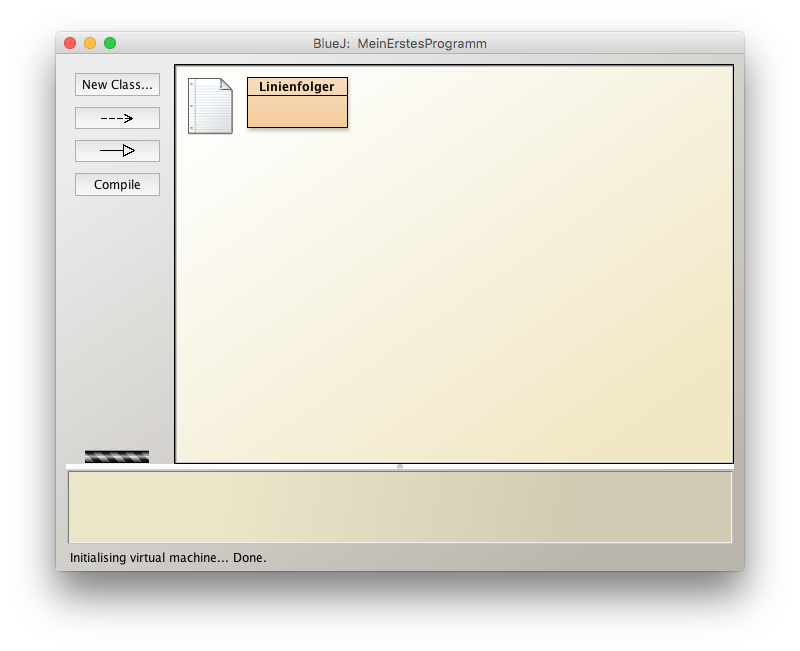
\includegraphics[scale=0.4]{images/firstprogram.png}
\caption{Die Benutzeroberfläche von BlueJ}
\label{fig:BlueJ UI}
\end{figure}

Nicht nur in den Universitäten wird BlueJ inzwischen als Werkzeug zur Einführung in die Programmiersprache Java und die objektorientierte Programmierung genutzt, auch im Schulkontext hat die intuitive Bedienung und übersichtliche Gestaltung Anklang gefunden, da BlueJ "`eine einfache Entwurfssicht für die Analyse gegebener Lösungen und für die Planung neuer Lösungen"' \cite[S.6]{ehmann:09} zur Verfügung stellt. Eine weitere Besonderheit besteht darin, dass im Gegensatz zu anderen Entwicklungsumgebungen -- im Gegensatz zu den meisten anderen Entwicklungsumgebungen -- in BlueJ "`schnell einige Objekte erzeugt und sofort untersucht werden"' \cite[S.6]{ehmann:09} können. Hierzu bietet BlueJ die \emph{Inspect-}Funktion an, die über das Kontextmenü eines erzeugten Objekts erreichbar ist, und die Werte der Feldvariablen genau dieses Exemplars einer Klasse anzeigt.

\begin{figure}[htpb]
\centering
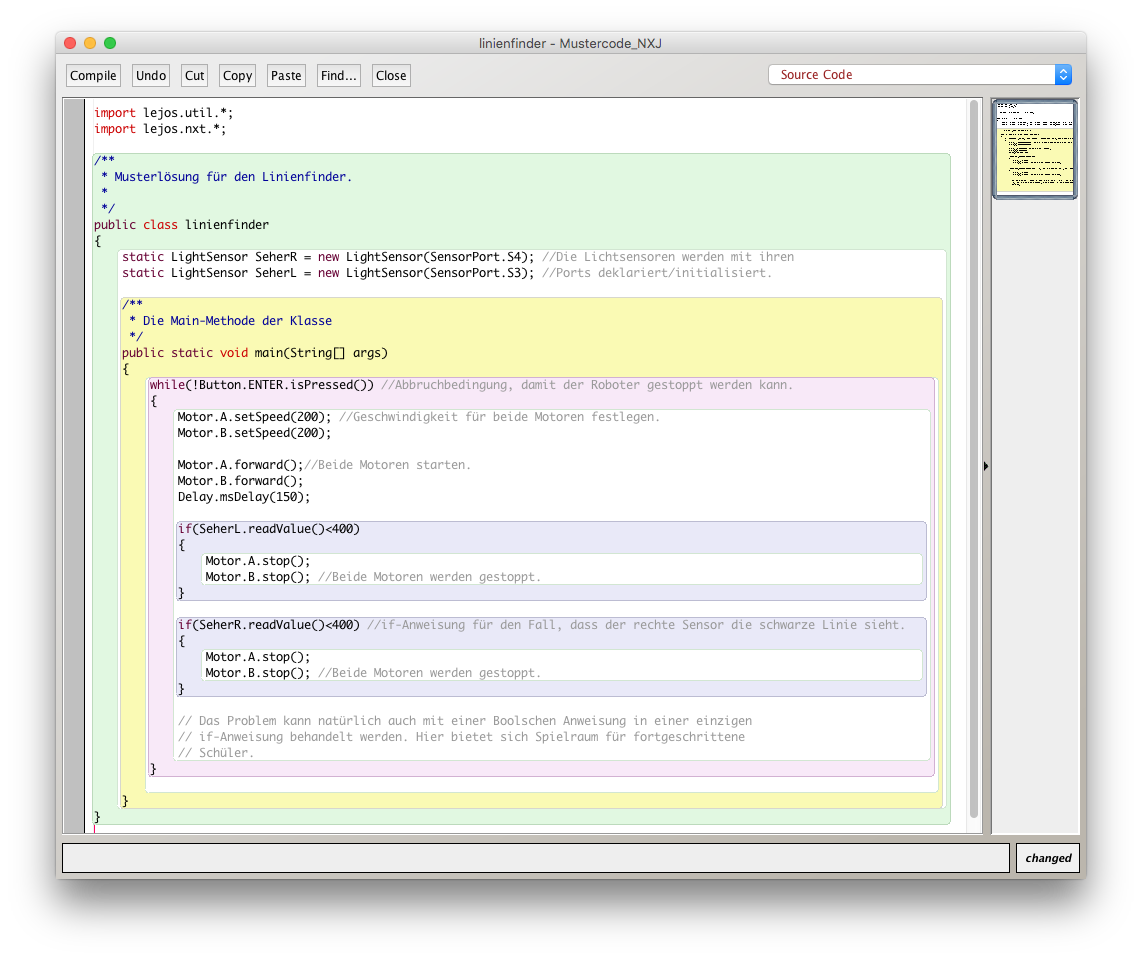
\includegraphics[scale=0.3]{images/linienfinder_bluej.png} 
\caption{BlueJ-Beispiel zum Finden einer Linie}
\label{fig:Bsp BlueJ Linienfinder}
\end{figure}


\par \singlespacing
\subsection{leJOS}
\label{sec:lejos}
\onehalfspacing
leJOS ist eine kleine Java Virtual Machine und stellt alle Klassen der NXJ API zu Verfügung, mithilfe derer \textsc{Lego Mindstorms} NXT Roboter in Java programmiert werden können (vgl. \cite{lejos}).\\
In der Kombination mit BlueJ ergibt sich somit für die SuS eine besonders einfache Softwarelösung. Durch eine eigens für BlueJ und NXT Roboter geschriebene sogenannte \textit{Extension} (siehe hierzu \cite{bowes:12}) und den Import der NXJ API stehen den SuS nicht nur die Klassen zur Steuerung ihres Roboters zur Verfügung. Darüber hinaus besteht Möglichkeit, über eine Erweiterung des Kontextmenüs, um spezielle Befehle, die dazu dienen, das in BlueJ geschriebene Programm auf den NXT-Stein zu übertragen. Dies steht allen in BlueJ geschriebenen Klassen zur Verfügung, wie in Abbildung \ref{fig:extension} sichtbar ist.
\pagebreak

Mithilfe von BlueJ (oder einer anderen Entwicklungsumgebung) können die SuS unter anderem kontextorientierte Aufgaben lösen. z Hierzu gehören zum Beispiel das Anhalten auf einer Linie (vgl. Abb. \ref{fig:Bsp BlueJ Linienfinder}) oder auch den Roboter einer schwarzen Linie folgen zu lassen, was eine der Grundaufgaben im RoboCup Junior Rescue Wettbewerb darstellt (vgl. Abb. \ref{fig:Bsp BlueJ Linienfolger}).

\begin{figure}[htbp]
\centering
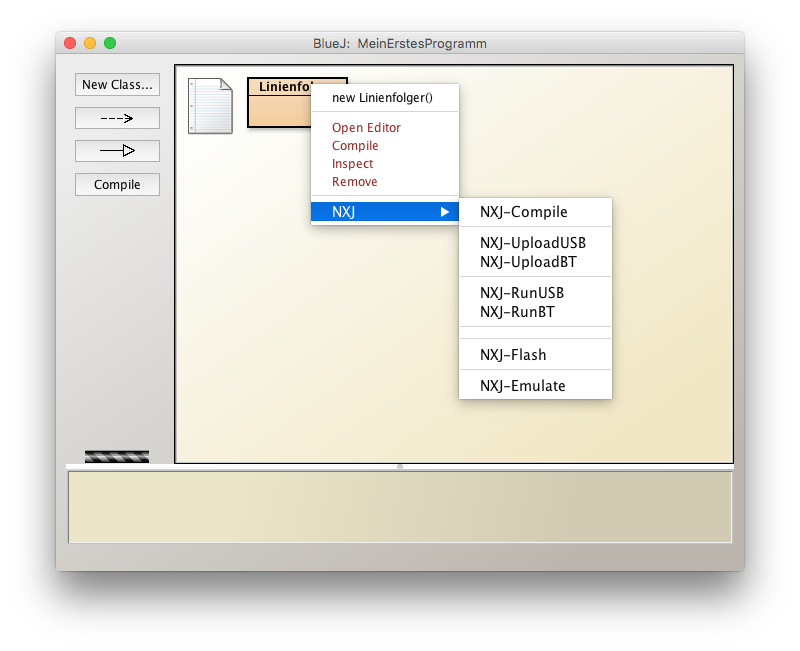
\includegraphics[scale=0.4]{images/extension.png}
\caption{Das Kontextmenü mit Auswahlmöglichkeiten der NXJ-Extension}
\label{fig:extension}
\end{figure}



\begin{figure}[htbp]
\centering
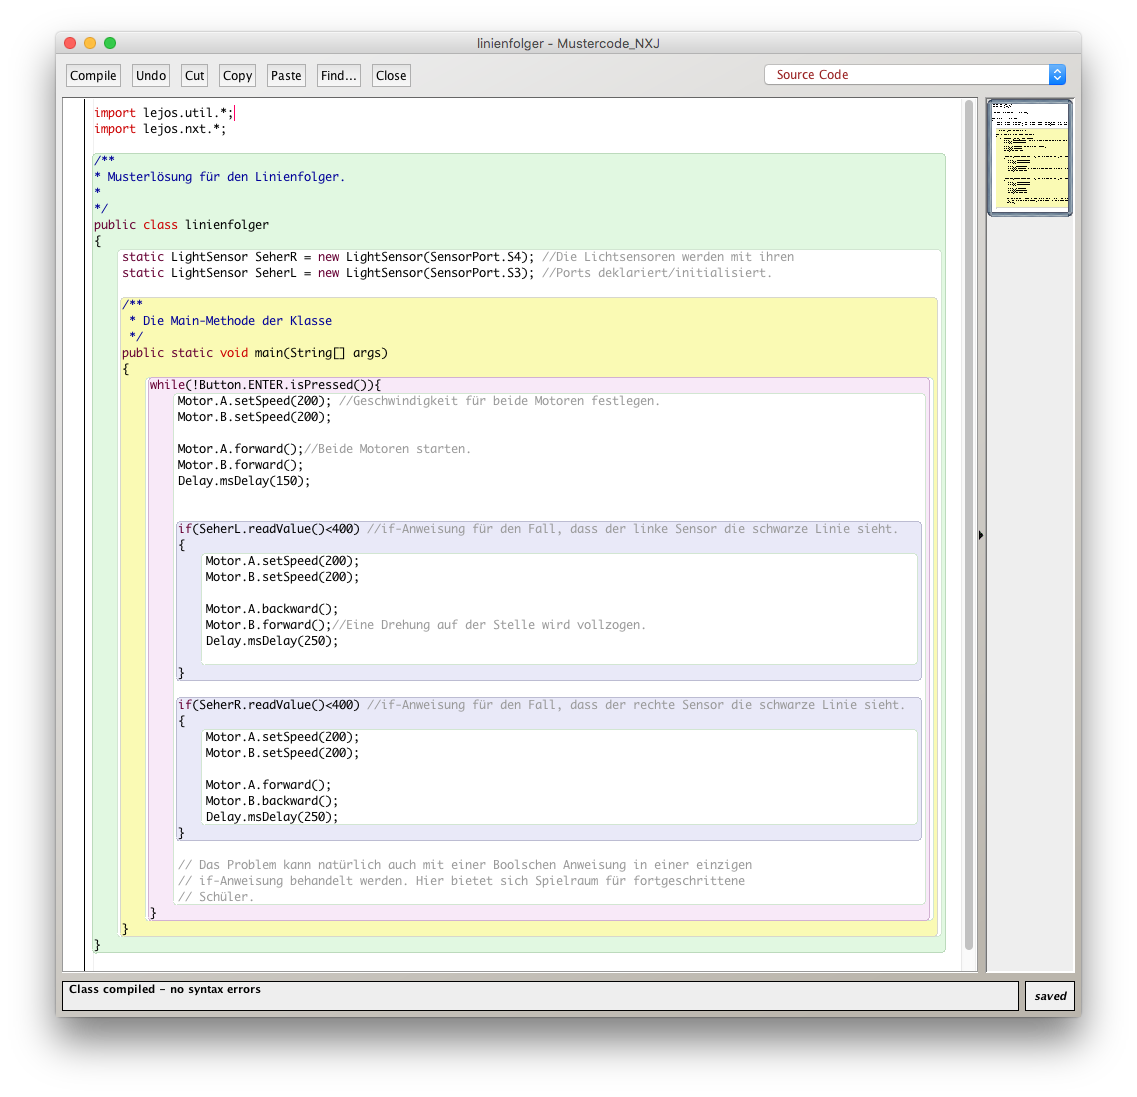
\includegraphics[scale=0.35]{images/linienfolger_bluej.png} 
\caption{Der Roboter soll einer schwarzen Linie folgen}
\label{fig:Bsp BlueJ Linienfolger}
\end{figure} 

Der Vorteil an der Arbeit mit leJOS besteht darin, dass die SuS direkt mit reinem Java-Code in Berührung kommen. Von Anfang an müssen sie auf syntaktische Korrektheit achten, damit ihr Programm überhaupt auf den NXT Roboter übertragen werden kann. Dabei stellen sich bereits mit wenigen zu lernenden Methoden schnell die ersten Erfolge ein: für das einfache Fahren eines Vierecks müssen die SuS lediglich die  Methoden \texttt{setSpeed()}, \texttt{forward()} und \texttt{backward()} an beiden Motoren, sowie eine Verzögerung mithilfe des Klasse \texttt{Delay} benutzen. 



\par \singlespacing
\section{Simulationsumgebungen}
\label{sec:simulationsumgebungen}
\onehalfspacing
Für den virtuellen Umgang mit \textsc{LEGO Mindstorms} Roboter jeder Generation gibt es bereits einige Simulatoren, die frei verfügbar sind.\\
Zunächst sollte in diesem Zusammenhang eine an der RWTH Aachen genutzte Simulationsumgebung erwähnt werden, in der sich ein Roboter in einer virtuellen 3D-Umgebung bewegen kann (vgl. \cite{rwth}). Diese ist für die Benutzung der Windows-Entwicklungsumgebung \emph{BricxCC} konzipiert, die unter anderem die an \textsc{LEGO} NXT Roboter angepasste Programmiersprache \emph{Not eXactly C (NXC)} (s. \cite{bricxcc}) unterstützt.

Des weiteren existiert \emph{nxcEditor}, eine sowohl mit Windows, als auch mit Linux und \mbox{MacOS} nutzbare Entwicklungsumgebung, die einen Simulator, \emph{nxcSimulator} beinhaltet. Ähnlich wie BricxCC nutzt auch der nxcEditor die Programmiersprache NXC (s. \cite{nxceditor}). Programmiert wurde die Entwicklungsumgebung von Frank Knefel und ist in Anlehnung an das vom Fraunhofer IAIS initiierte Lehr-/Lernkonzept \emph{Roberta -- Lernen mit Robotern} konzipiert. Deshalb wird die erwähnte Entwicklungsumgebung inzwischen auch direkt von Roberta als Softwarelösung angeboten wird (vgl. \cite{roberta}).

Abschließend ist noch das umfassende Softwareangebot des Virtuellen Campus Projekts der PHBern zu erwähnen. Dieses umfasst -- neben der Entwicklung von Programmen für \textsc{LEGO Mindstorms} NXT Roboter mithilfe einer eigens für NXT Roboter geschriebenen Klassenbibliothek \emph{NxtJLib} (s. \cite{aegidius:16}) -- die Möglichkeit, das Programm auf verschiedene Weisen auf den NXT-Stein zu übertragen, oder in einem Simulator auszuprobieren (s. \cite{phbern}). 

\par \singlespacing
\chapter{Anforderungen an die Neuimplementierung}
\label{chap:anforderungen}
\onehalfspacing
Nicht nur in der Schule, sondern insbesondere in der Wissenschaft spielt Simulation in der Robotik eine wichtige Rolle \cite[S.13]{hertzberg:12}. Die Anforderungen, die an die wissenschaftlichen Simulationsumgebungen der Robotik gestellt werden, fassen \textsc{Hertzberg, Lingemann} und \textsc{Nüchter} wie folgt zusammen:
\begin{quote}
\begin{itemize}
\item "`Die Umgebung muss hinreichend gut simuliert sein. Die Simulation einer Flughafenterminalhalle muss zum Beispiel "`zufällig"' umherlaufende Fluggäste mit Gepäck und Transportkarren umfassen.

\item Der Roboter in seiner Funktionalität muss hinreichend gut simuliert sein. Das betrifft seine Aktionen wie auch seine Sensorik.

\item Relevante Ungenauigkeit technischer Sensoren und Effektoren muss abgebildet werden. Kann zum Beispiel im realen Bild einer Kamera auf dem Roboter ein Orientierungspunkt im Gegenlicht der Fensterfront unsichtbar werden, muss die Simulation diesen Effekt reproduzieren.

\item Die "`Wahrheit"' im Simulator ist tabu! Natürlich ist im Simulator der Zustand jedes simulierten Objekts präzise bekannt, einschließlich der Position, Richtung und Geschwindigkeit des Roboters. Die Roboterkontrollsoftware darf hierauf nicht zugreifen, um Information über die Umgebung zu erhalten -- das geht nur über die simulierten Sensoren. (Für die externe Bewertung des Roboterverhaltens ist der Vergleich zwischen der Wahrheit im Simulator und der Information in der Roboterkontrollsoftware aber erlaubt.)

\item Der Simulator sollte für den simulierten Roboter die identische Schnittstelle wie der reale Roboter zwischen Roboterkontrollsoftware einerseits und Robotersensorik und -aktuatorik andererseits verwenden; die Roboterkontrollsoftware soll also code-identisch für den realen oder den simulierten Roboter verwendet werden."' \cite[S.14]{hertzberg:12} 
\end{itemize}
\end{quote}

Im Hinblick auf die Entwicklungs einer Simulationsumgebung für die Schule sind mehrere Perspektiven von Belang. 
In den folgenden beiden Unterkapiteln werden nun die Anforderungen an die Neuimplementierung des Simulator-Prototyps für \textsc{LEGO Mindstorms} NXT Roboter aus Sicht der Schüler und der Lehrer dargestellt. Zudem wird geklärt, inwiefern die wissenschaftlichen Anforderungen aus dem universitären Bereich, wie oben dargestellt, auch auf die schulische Lehre zutreffen und wie diese gegebenenfalls angepasst werden müssen.

\par \singlespacing
\section{Schülerperspektive}
\label{sec:schüler}
\onehalfspacing

Da es sich bei der Simulationsumgebung um einen Prototypen handelt, der möglicherweise schon ab der fünften, regelmäßig aber ab der siebten Klasse eingesetzt werden soll, steht ein Augenmerk ganz besonders im Fokus: die Einfachheit. Sowohl in der Bedienung des Simulators als auch im Aussehen sollten klare und leicht erkennbare Strukturen vorherrschen.

Des weiteren sollte darauf geachtet werden, dass die SuS für die Programmierung des Roboters und die Benutzung des Simulators eine einheitliche Syntax verwenden können. Hierzu muss die Simulationsumgebung genau die Methoden anbieten, die auch bei dem realen Roboter die Steuerung der Motoren und den Zugriff auf Sensordaten ermöglichen. Dies entspricht dem zweiten Aspekt nach \textsc{Hertz\-berg\-/\-Lin\-ge\-mann\-/Nüch\-ter}, da der simulierte Roboter alle für die Arbeit mit SuS zentralen Funktionen anbieten und sich hinreichend ähnlich wie ein Roboter in der Realwelt verhalten soll. Des weiteren wird hiermit auch der Aspekt der code-identischen Roboterkontrollsoftware erfüllt, da die SuS das selbe Programm für den Simulator, wie auch für die Steuerung des Roboters selbst benutzen können sollten.

Ein weiterer Aspekt, den \textsc{Hertz\-berg\-/\-Lin\-ge\-mann\-/Nüch\-ter} beschreiben sind die Parcours. Diese sollten möglichst realitätsgetreu umgesetzt werden. Das heißt, dass Ausschnitte eines bestehenden realen Wettbewerbsparcours genutzt werden könnten, um für die SuS eine möglichst realitätsnahe Testumgebung anzubieten. Der Vorteil darin besteht auch in der Vergleichbarkeit der Ergebnisse. Die SuS lernen gleich zu Beginn einen wichtigen Aspekt bei der Entwicklung von Code für Roboter: nur weil der Roboter im Simulator an einer schwarzen Linie entlangfahren kann, bedeutet dies nicht, dass auch der reale Roboter diese Herausforderung problemlos meistert.


\par \singlespacing
\section{Lehrkraft}
\label{sec:lehrkraft}
\par \onehalfspacing
Für Lehrkräfte ist es erfahrungsgemäß wichtig, dass die Simulationsumgebung alle essentiellen Bausteine der objektorientierten Programmierung im Kontext der \textsc{LEGO} Roboter zur Verfügung stellt. Hierzu gehört das Austesten des Fahrens mithilfe einer Schleife, sowie der verschiedenen Sensoren. Dafür sollte es eine Auswahl an verschiedenen Parcours geben, damit der Fokus bei jedem Parcours auf einer einzigen Sache liegt. Sollen etwa die angebauten Lichtsensoren getestet werden, so bietet es sich an, den Parcours einfach aus einem weißen Hintergrund und einer schwarzen Linie, die entweder senkrecht in der Nähe des Roboters platziert ist, oder als Kurve eine Teilstrecke des realen Labyrinths darstellt, bestehen zu lassen.\\
In diesem Zusammenhang sollte die Möglichkeit gegeben sein, dass Lehrkräfte unter bestimmten Voraussetzungen eigene, an ihren Unterricht angepasste Parcours in die Software einbinden können.

Des weiteren ist es wichtig, dass sich Lehrerinnen und Lehrer schnell in die Simulationsumgebung einarbeiten können, um bei Fragen der SuS sofort Hilfe leisten zu können. %Hier kann die Einbindung in BlueJ als klarer Vorteil gesehen werden.\\


% Hierzu wird ein einheitlicher Startpunkt des Roboters im Parcours von der Software festgelegt und in einer Kurzanleitung niedergeschrieben.

\par \singlespacing
\section{Erweiterbarkeit} \label{sec:erweiterbarkeit}
\onehalfspacing
Nun zu dem Aspekt der Erweiterbarkeit, der für die Entwicklung dieser Simulationsumgebung -- insbesondere, da diese für den Einsatz in Schulen konzipiert ist -- zentral ist.

Zunächst sollte die Software ausreichend kommentiert werden, damit auch nach Fertigstellung dieser Masterarbeit weitere Module hinzugefügt werden können. Dazu gehören insbesondere einige Arten von Sensoren, die in diesem Prototyp nicht realisiert wurden. Aber auch Änderungen, die im Rahmen von Veränderungen der leJOS NXJ API stattfinden, müssen berücksichtigt werden können.

Leider hat sich während der Entstehung dieser Simulationsumgebung herausgestellt, dass der Verkauf von \textsc{LEGO Mindstorms} NXT Robotern zum 31.12.15 eingestellt wurde. Dies bedeutet, dass im Hinblick auf die Entwicklung der Robotik in Schulen auch die Möglichkeit, die geschriebene API an die Technologie der \textsc{LEGO Mindstorms} EV3, den Nachfolge-Robotern der NXT, anzupassen, essentiell ist.


\par \singlespacing
\chapter{Entwickelte Software}
\onehalfspacing
\par \singlespacing
\section{Prozesse während der Implementation}
\onehalfspacing
Die Entwicklung des Prototyps der Simulationsumgebung umfasste mehrere Schritte, sowie einige Vorarbeit. Diese werden im folgenden Abschnitt nun kurz zusammengefasst.
\par \singlespacing
\subsection{Mock-Ups} 
\onehalfspacing
Um einen visuellen Grundgedanken festzuhalten und das Ziel der Implementation der vollständigen Simulationssoftware zu erfassen wurden zunächst Skizzen angefertigt, die einen groben Überblick über die Benutzeroberfläche geben sollten. Diese enthielten eine beispielhafte Darstellung eines Parcours und eines Roboters, sowie eine Menüzeile am oberen Rand. Als nächstes wurden eine spezielle Art von Interaktionsprototypen hergestellt, so genannte \emph{interaktive Mock-Ups}, die eine Subkategorie interaktiver Wireframes darstellen. Interaktive Wireframes sind eine vereinfachte, digitale Darstellung von Benutzerschnittstellen, die einen gewissen Grad an Interaktionslogik umfassen (vgl. \cite[S.162ff.]{moser:12}).\\
 Hierzu wurde mit der Software \emph{Axure RP Pro} gearbeitet, mit der sich sowohl einfache als auch komplex verschachtelte Mock-Ups erstellen lassen (s. Abb.\ref{fig:axure}).

\begin{figure}[htbp]
\centering
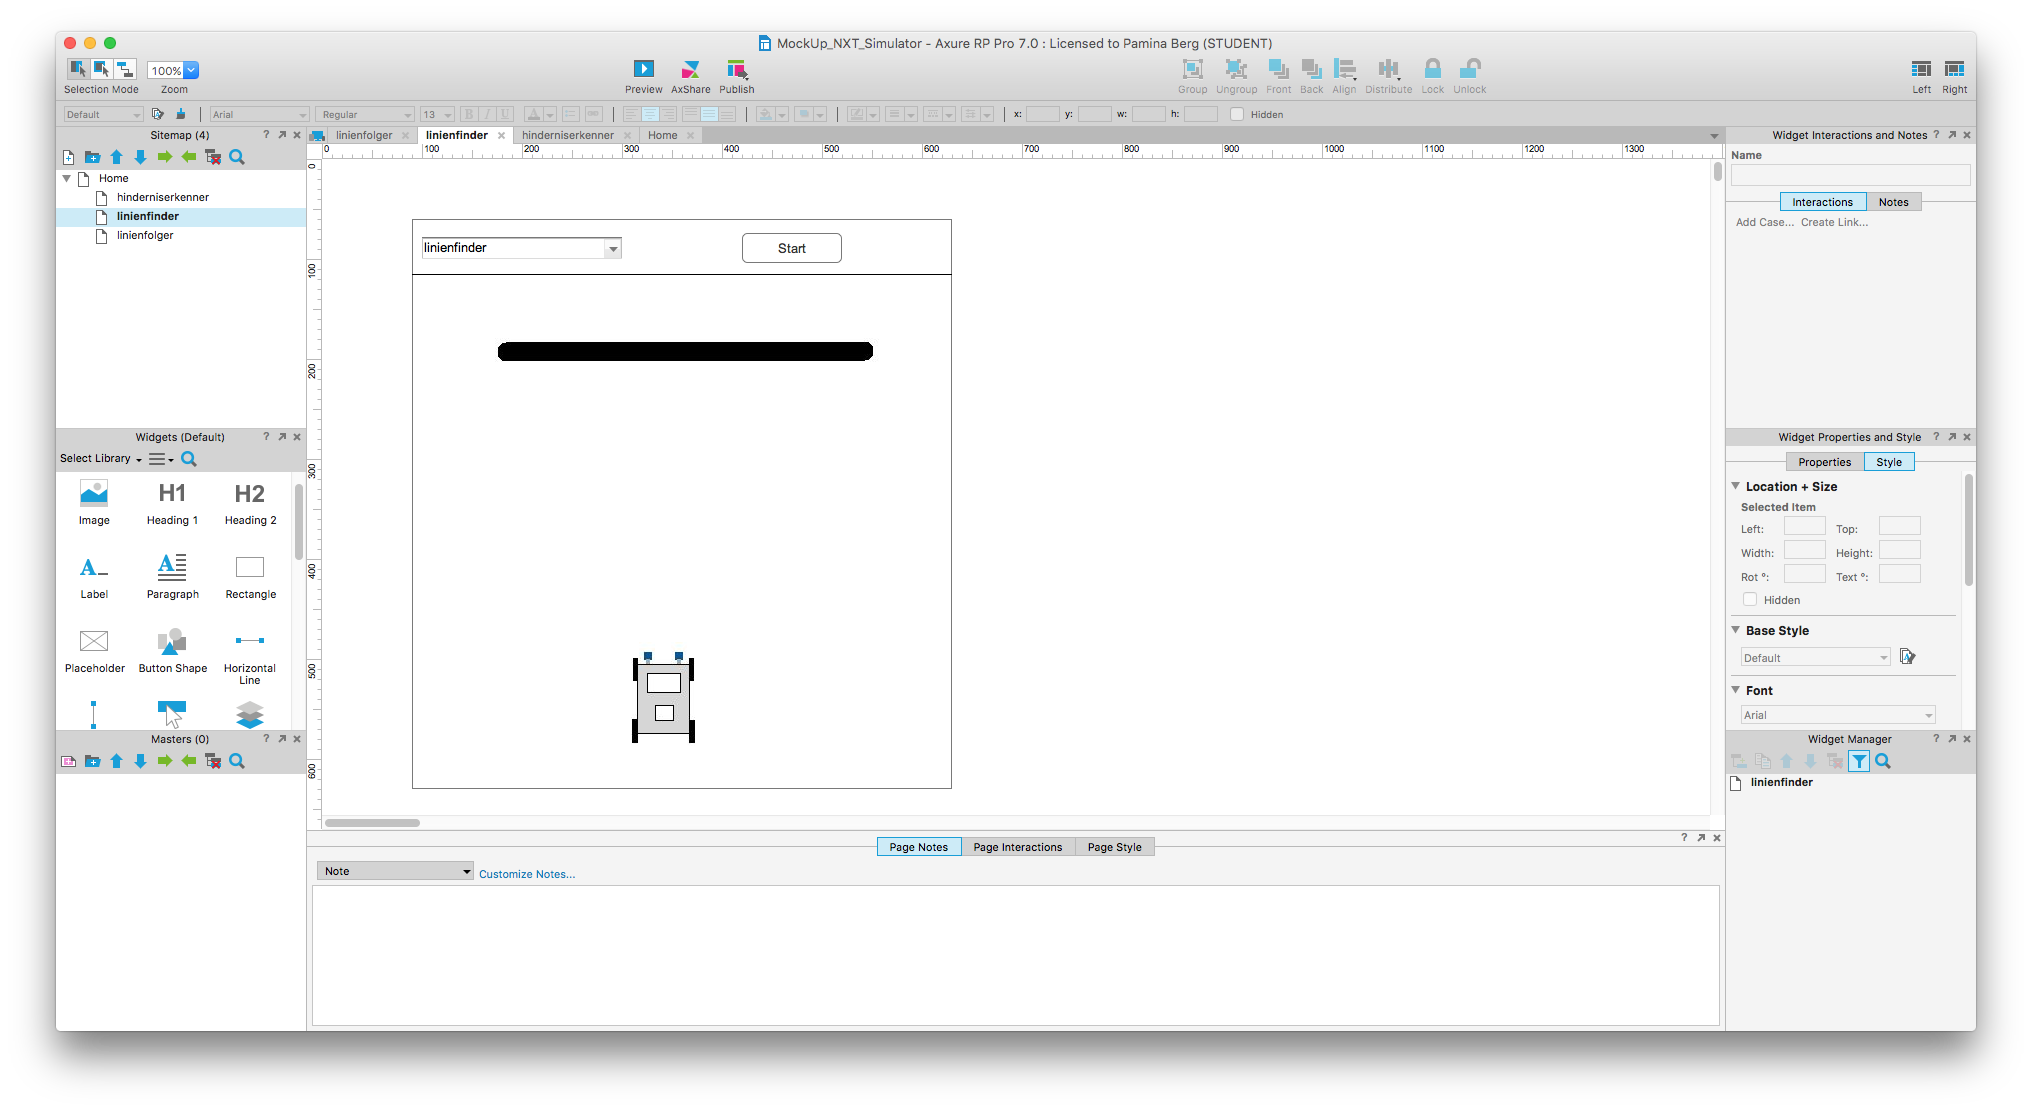
\includegraphics[scale=0.2]{images/axure_mockup.png} 
\caption{Die Bedieneroberfläche von Axure RP Pro}
\label{fig:axure}
\end{figure}


%Da die zu schreibende API auch mehrere Sensoren umfasst, sollten die in den Mock-Ups dargestellten Szenarien den für den Schulkontext erforderlichen Funktionsumfang repräsentieren. Hierzu gehörte das Anhalten auf einer schwarzen Linie wie in Abbildung \ref{fig:linienfinder}, das Fahren entlang einer schwarzen Linie (s. Abb. \ref{fig:linienfolger}) und das Finden und Umfahren eines Hindernisses auf der Fahrbahn (s. Abb. \ref{fig:hinderniserkenner}).

\begin{figure}[htbp]
\centering
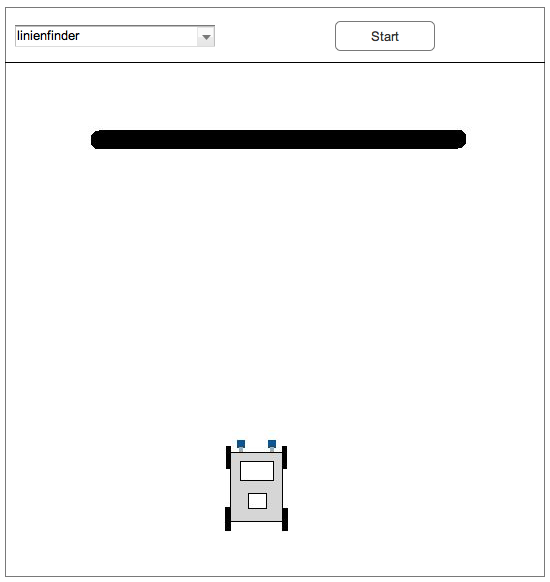
\includegraphics[scale=0.4]{images/mockup_linienfinder.png}
\caption{Anhalten auf einer schwarzen Linie}
\label{fig:linienfinder}
\end{figure}

\begin{figure}[htbp]
\centering
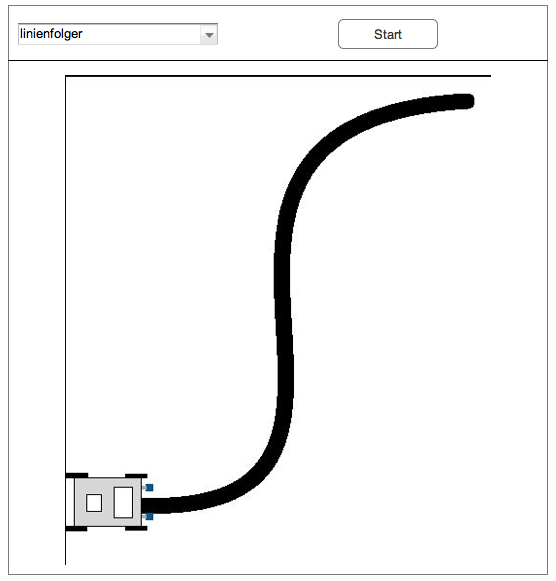
\includegraphics[scale=0.4]{images/mockup_linienfolger.png}
\caption{Fahren einer S-Kurve}
\label{fig:linienfolger}
\end{figure}

\begin{figure}[htbp]
\centering
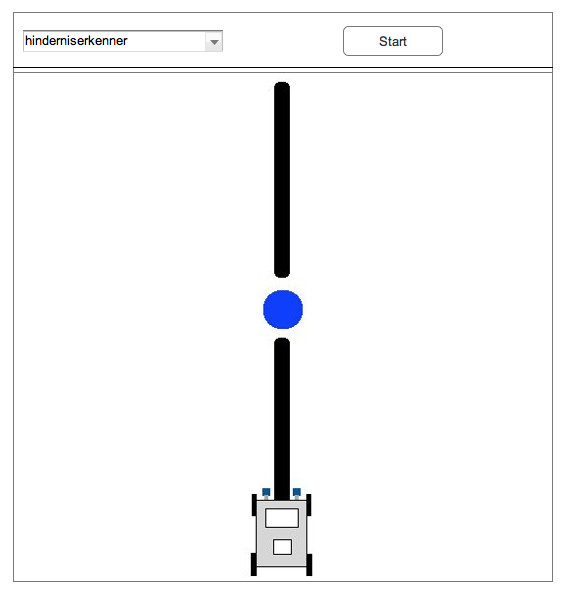
\includegraphics[scale=0.4]{images/mockup_hinderniserkenner.png}
\caption{Erkennen eines Hindernisses auf der Fahrbahn}
\label{fig:hinderniserkenner}
\end{figure}
\par \singlespacing
\subsection{Schritte während der Implementation}
\onehalfspacing
Nach dem Erstellen der Mock-Ups musste nun überlegt werden, inwiefern die vorherigen Überlegungen umgesetzt werden konnten. Die erste Abstraktion, die während den ersten Implementationsschritten stattgefunden hat, war die Darstellung des Roboters in der Umgebung, sodass dieser einfach als Dreieck implementiert wurde. 

Außerdem konnte bestehender Code aus anderen Projekten in dieses Projekt importiert werden. So wurde die leJOS API, deren Klassen im Paket der Klassenbibliothek frei verfügbar sind, genutzt, um die Neuimplementation der in \textbf{\ref{sec:API}} beschriebenen Klassen realitätsgetreu miteinander zu verzahnen und die korrekten Beziehungen untereinander zu implementieren.

\par \singlespacing
\subsection{Integration in BlueJ}
\label{sec:integration}
\onehalfspacing
Die Frage nach einer Integration in BlueJ kann auf vielfältige Art beantwortet werden. Die einfachste und zu diesem Zeitpunkt praktikabelste Lösung ist, die Integration der Simulationsumgebung über einen Import der Klassenbibliothek zu realisieren.\\
Für die SuS bedeutet dies, dass diese, neben der Import-Anweisung für die leJOS-Bibliothek zwei weitere Import-Anweisungen in ihren geschriebenen Code einfügen müssen. Außerdem muss ein Exemplar der Simulator-Klasse erzeugt werden. Da dies aber ein überschaubarer Aufwand für SuS und Lehrkraft ist, der auch als "`Schablone"' für die ersten Versuche von der Lehrkraft zur Verfügung gestellt werden kann, sehe ich diese Lösung als geeignet an.

Nun kann man sich die Frage stellen, wieso überhaupt mit BlueJ gearbeitet werden soll, da es doch ausreichend andere Entwicklungsumgebungen gibt, in die solche Bibliotheken importiert werden können.\\
Der Vorteil an BlueJ besteht darin, dass diese Entwicklungsumgebung, wie in \textbf{\ref{sec:bluejetc}} beschrieben, eine klar strukturierte und übersichtliche Benutzeroberfläche bietet. Die SuS müssen sich nicht in für ihre Ansprüche überdimensional umfangreiche Programmierumgebungen einarbeiten und können per Mausklick ihren Code per USB-Kabel auf den Roboter übertragen. Dies wird von einer speziell für BlueJ entwickelten NXT-Extension  (vgl. \cite{bowes:12}), die eine Erweiterung des Kontextmenüs jeder Klasse zur Verfügung stellt, realisiert.

\par \singlespacing
\section{Beschreibung der Software}
\onehalfspacing

Nun zu einer kurzen Beschreibung des Prototyps, in der zudem Einzelheiten zur Benutzung der Software dargestellt werden.



\begin{figure}[H]
\centering
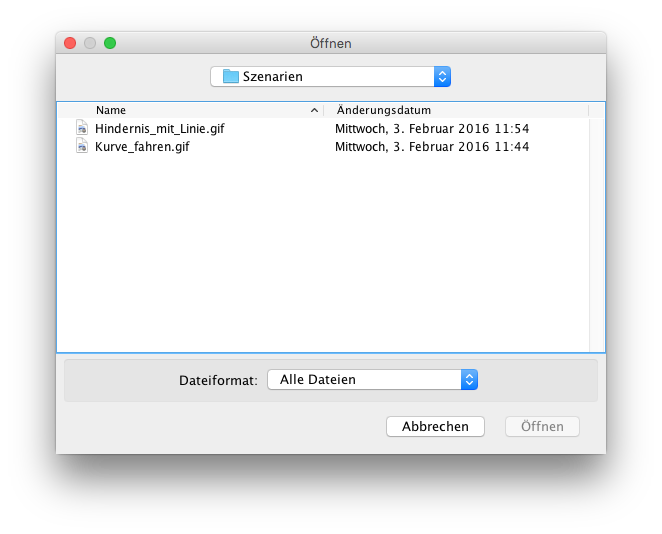
\includegraphics[scale=0.45]{images/dialog_szenarien.png} 
\caption{Auswahldialog für den Parcours}
\label{fig:auswahldialog}
\end{figure}
Beginnt man mit dem Programmieren einer Klasse, die den NXT Roboter beispielsweise einer Kurve auf dem Boden folgen lassen soll, so müssen neben des Imports für die leJOS API zwei weitere Import-Anweisungen für den Simulator eingebunden werden. Diese Klasse sei im Folgenden mit \texttt{linienfolger} bezeichnet.\\
Zu beachten ist, dass immer entweder der leJOS-Import oder die Simulator-Importe auskommentiert sein müssen, da sonst weder der Simulator noch der reale NXT Roboter weiß, auf welche Bibliothek zugegriffen werden soll.

Um nun mit dem Simulator zu arbeiten, erzeugt man innerhalb der main-Methode der Klasse \texttt{linienfolger} ein neues Exemplar der Klasse \texttt{Simulator}. Nachdem man die Klasse \texttt{linienfolger} fehlerfrei kompiliert hat, kann man in BlueJ über einen Rechtsklick ein neues Exemplar dieser Klasse aufrufen, und an diesem die main-Me\-tho\-de ausführen lassen. Dies führt dazu, dass mit der Erzeugung eines Simulators der Auswahldialog für den Parcours angezeigt wird, wie in Abbildung \ref{fig:auswahldialog} beispielhaft dargestellt ist.\\
Sobald der Parcours ausgewählt wurde, wird dieser in einem neuen Fenster geöffnet. Nun sehen die SuS den Roboter, der auf dem von ihnen ausgewählten Parcours fährt (Vgl. Abb.\ref{fig:simparcours_kurve}).

\begin{figure}[htbp]
\centering
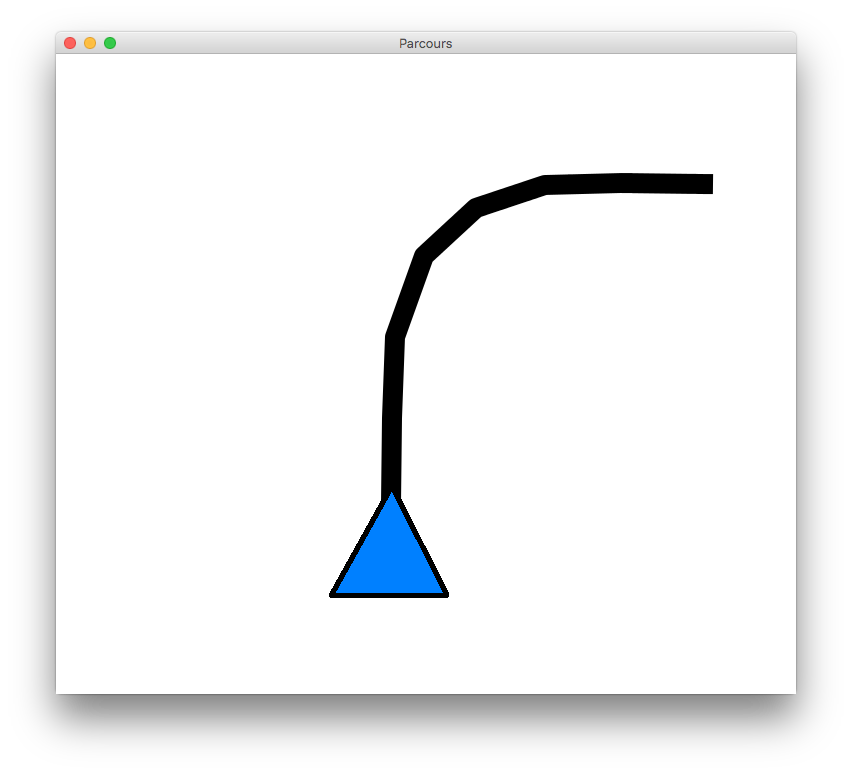
\includegraphics[scale=0.45]{images/simparcours_kurve.png} 
\caption{Eine beispielhafte Darstellung von Parcours und Roboter}
\label{fig:simparcours_kurve}
\end{figure}


\par \singlespacing
\section{Softwarearchitektur}
\onehalfspacing 

Die entwickelte Software besteht im derzeitigen Zustand als Prototyp aus insgesamt fünfzehn Klassen. Diese sind zur Übersichtlichkeit in Pakete unterteilt. Diese unterscheiden sich in zwei Kategorien. Zum einen die Klassen, die die API für den Simulator zur Verfügung stellen und die zentralen von leJOS angebotenen Klassen für die NXT-Roboter umfassen, zum anderen die Klassen, die für die Repräsentation der Simulation auf dem Bildschirm zuständig sind. Um eine Konsistenz bei den Imports für die SuS zu bewahren, sind die Klassen, die die simulierten NXT-Teile implementieren, in einem Package mit der Bezeichnung \texttt{nxt} (ähnlich wie bei leJOS) enthalten, die Klassen des Simulators in dem Package \texttt{sim}. 

Zum besseren Verständnis nun eine kurze Zusammenfassung der in dieser Implementation verwendeten Projektstruktur.

\subsubsection*{Pakete}

Pakete in Java, auch \emph{packages} genannt, fassen Gruppen von Typen zusammen. Ein Beispiel hierfür sind die Standardbibliotheken von Java, die in den Paketen \texttt{java} und \texttt{javax} zu finden sind. Diese enthalten Unterpakete, wie zum Beispiel die Bibliotheken zur Entwicklung grafischer Benutzeroberflächen \emph{Swing} oder auch \emph{AWT} (vgl. \cite[S.265]{ullenboom:12}).
Der Zugriff auf diese Bibliotheks-Klassen erfolgt entweder über eine Pfadangabe bei der Variablendeklaration und -initialisierung oder über eine \texttt{import}-Anweisung. Will man beispielsweise ein Exemplar der Klasse \texttt{Point} aus der Java-Klassenbibliothek \texttt{AWT} erzeugen, so kann dies entweder durch den Befehl \texttt{java.awt.Point Punkt = new java.awt.Point();} statt der "`normalen"' Deklaration und Initialisierung, oder aber durch die Anweisung \texttt{import java.awt.Point;} zu Beginn des Quelltexts geschehen (vgl. \cite[S.266]{ullenboom:12}).
Möchte man eine ganze Reihe von Klassen eines Pakets importieren, so besteht die Möglichkeit, dies mithilfe eines * am Ende der Import-Deklaration zu tun. Im obigen Beispiel wäre dies \texttt{import java.awt.*;}. Anhand dieser Deklaration ist auch direkt zu erkennen, dass das Paket \texttt{awt} ein Unterpaket des Pakets \texttt{java} ist. Der "`Paketpfad"' bzw. die hierarchische Struktur der Pakete und Unterpakete wird mithilfe von Punkten angegeben (vgl. \cite[S.265ff.]{ullenboom:12}, \cite[S.84ff.]{abts:15}).

\subsection{Externe Frameworks}

\subsubsection*{AWT}

Die Klassenbibliothek AWT (\emph{Abstract Window Toolkit}) stellt die grundlegenden Bausteine zur Erstellung grafischer Benutzeroberflächen zur Verfügung. Die Darstellung von AWT-Komponenten ist an die Darstellungoptionen des jeweiligen Betriebssystems gekoppelt, wodurch eine Eingrenzung der Möglichkeiten auf diejenigen, die auf alle Betriebssysteme zutreffen, vorhanden ist. Vorteilhaft dabei ist, dass das Erscheinungsbild von Menüleisten und Schaltflächen dem Benutzeroberflächendesign des Betriebssystems entspricht (vgl. \cite[S.279]{abts:15})\\
Auf einem anderen Konzept bauen die Klassen des Pakets \emph{Swing} auf. 

\subsubsection*{Swing}

Das Paket \texttt{javax.swing} basiert fast vollständig auf Java und ersetzt alle Grundkomponenten des AWT-Frameworks. Im Gegensatz zu AWT wird hier auf die Designkonsistenz zum Betriebssystem verzichtet. Im Gegenzug bekommt man ein einheitliches und plattformunabhängiges \emph{Look \& Feel} (vgl. \cite[S.279]{abts:15}). Dies ist darin begründet, dass die Swing-Komponenten mit "`primitiven Zeichenoperationen gemalt"' werden \cite[S.1018]{ullenboom:12}.


\subsubsection*{ImageIO}

Das Paket \texttt{java.imageio} bietet dem Benutzer Schnittstellen zur Einbindung von Bilddateien in Java an. Hierzu gehört unter anderem das Lesen und Schreiben von Bildern in unterschiedlichen Formaten \cite[S.1280]{ullenboom:12}. Mithilfe der Methode \texttt{ImageIO.read(URL input)} wird ein Bild aus dem übergebenen Verzeichnis oder der URL direkt in das Projekt geladen. 


\par \singlespacing
\subsection{Die Klassen des \texttt{nxt}-Package}
\label{sec:API}
\onehalfspacing
In diesem Abschnitt werden nun die von leJOS vorgegebenen und für die Implementation des Simulators angepassten Klassen vorgestellt. Hierbei handelt es sich um eine kleine Auswahl der essentiell für den Unterricht erforderlichen Klassen, die im Rahmen dieser Arbeit für den Prototyp angepasst wurden. Die interne Struktur zwischen den einzelnen Klassen ist durch die leJOS API vorgegeben und musste somit realitätsgetreu nachgebildet werden (Vgl. Abbildung \ref{fig:api_uml}).

\subsubsection{Motoren}
Zunächst wurde die Klasse \texttt{Motor} implementiert. Diese besteht lediglich aus den Feldern \texttt{A, B} und \texttt{C}, die Exemplare der Klasse \texttt{NXTRegulatedMotor} darstellen. Ein NXTRegulatedMotor ist ein an einen Motorport angeschlossener NXT-Motor. Ein solcher Motor wird über den Befehl \texttt{Motor.[port].[Methode]} angesteuert. 

\subsubsection{MotorPort}
Die Klasse \texttt{MotorPort} ist in diesem Projekt eine verkleinerte Version der gleichnamigen Klasse aus der leJOS API. In ihr sind die statischen Variablen \texttt{A, B} und \texttt{C} enthalten, die die zur Verfügung stehenden MotorPorts am Roboter darstellen. Intern ist jedem Port eine \texttt{id} in Form eines Integer zugeordnet. Über die Methode \texttt{get\-In\-stance(int id)} kann über die private Variable \texttt{id} der öffentliche Port (\texttt{A, B} und \texttt{C}) abgefragt werden.

\subsubsection{NXTRegulatedMotor}
In der Klasse \texttt{NXTRegulatedMotor} befindet sich die auf die Simulationsumgebung angepasste Implementation der NXT-spezifischen Motoren. Den größten Anteil haben hierbei Bewegungen der beiden Motoren über die Methoden \texttt{for\-ward()} und \texttt{back\-ward()}, sowie die Geschwindigkeitsregulierung über die Methode \texttt{set\-Speed()}. 

Jeder NXTRegulatedMotor ist an einen MotorPort angeschlossen, durch welchen eindeutig zuzuordnen ist, welcher Motor gerade angesprochen werden soll. Dies wird im Prototyp durch eine Feldvariable \texttt{{\_}port} gelöst, über die dann abgefragt werden kann, an welchem Motor gerade eine Methode aufgerufen wird. Folglich ist jedes NXT\-Regulated\-Motor\--Objekt ein Exemplar der Klasse NXTRegulatedMotor, welches vom Benutzer einen Port zugeordnet bekommt.\\
Zudem bekommt jeder Motor eine Feldvariable \texttt{{\_}richtung}, die die Information enthält, ob der Motor sich bewegt (vorwärts oder rückwärts), oder ob er gerade in Ruheposition ist. Dabei entspricht "`vorwärts"' der Zahl 1, "`rückwärts"' dem Wert -1 und mit 0 wird der Ruhezustand bezeichnet.

Die SuS werden ihren geschriebenen Code meist damit beginnen, den beiden Motoren jeweils eine Geschwindigkeit zuzuweisen. Dies geschieht mithilfe der Methode \texttt{setSpeed(int speed)}. Da sich der Roboter auf dem Parcours pixelweise bewegt, wird an dieser Stelle die Geschwindigkeit von den für reale NXT-Roboter geeigneten Geschwindigkeiten durch den Faktor 100 geteilt, um eine angemessene Bewegungsgeschwindigkeit auf dem Bildschirm zu sichern.\\
Danach werden die Motoren in Bewegung versetzt. Hierzu werden die Methoden\\
\texttt{forward()} und \texttt{backward()} benutzt. In der Implementation des Prototyps wird nun diese Bewegung als Veränderung der Position und der Ausrichtung der Roboter-Grafik auf der Leinwand realisiert. Je nachdem, welcher Port (\emph{B} entspricht dem linken Motor, \emph{C} dem rechten) angesteuert wird, ruft die Klasse NXTRegulatedMotor die Methode \texttt{aendereBewegung(double winkel, double geschwindigkeit)} am Roboter, in Abhängigkeit zur Geschwindigkeit und eines Richtungsmultiplikators, auf. Der Richtungsmultiplikator sorgt hierbei für eine möglichst realitätsnahe Approximation der tatsächlichen Veränderung der Ausrichtung des Roboters. Die Verwendung einer Variablen für diesen Faktor bringt den Vorteil mit sich, dass bei Verbesserungen innerhalb der Bewegungsimplementation der Motoren eine Konsistenz in allen involvierten Methoden sichergestellt ist. Soll beispielsweise die Vorwärtsbewegung der Motoren neu skaliert werden, so kann dies über die Veränderung des Richtungsmultiplikators geschehen und es werden in der Konsequenz alle relevanten Werte in den Methoden gleichzeitig und gleichmäßig verändert. 

Die Herausforderung bei diesem Prototyp bestand nun darin, dass die Motoren, auch wenn sie sich schon bewegen, eine neue Geschwindigkeit weitergegeben bekommen und die zuvor bestimmte Bewegung mit der neuen Geschwindigkeit ausführen. Außerdem sollte ein zweimaliges Aufrufen der Methoden \texttt{forward()} und \texttt{backward()} nicht dazu führen, dass der Roboter sich doppelt so schnell bewegt. Hierzu konnte nun die Information, die in  \texttt{{\_}richtung} enthalten ist, genutzt werden. Mit einfachen if-Abfragen wird zu Beginn des Methodenrumpfs festgestellt, in welcher Bewegung sich der angesprochene Motor gerade befindet. 


\subsubsection{Licht- und Farbsensoren}
Die Lichtsensoren sind zwei von der leJOS API vorgegebene Exemplare der Klasse \texttt{LightSensor}. Diese sind im Prototyp der Simulation jeweils links und rechts neben der Spitze des Roboter-Dreiecks angebracht (siehe hierzu Abb. \ref{fig:roboter_abstrakt}). Die Berechnung hierzu sehen wie folgt aus:

Für die Berechnung der Position des rechten Lichtsensors gilt:\\
Sei $B$ die Breite, $H$ die Höhe und $u$ die Ausrichtung des Roboters. Seien mit $xPos$ und $yPos$ die Koordinaten des Robotermittelpunkts bezeichnet. Dann gilt
\renewcommand\arraystretch{3}
\begin{align*}
\beta & = \arctan \left( \dfrac{\frac{B}{4}}{\frac{H}{2}} \right)\\
\epsilon & = 90 - (u + \beta)\\
c & = \left( \frac{B}{4} \right) \cdot \arcsin (\beta)\\
x_B & = xPos + \left( c \cdot \sin(\epsilon) \right)\\
y_B & = yPos - \left( c \cdot \cos(\epsilon) \right).
\end{align*}

Für die Berechnung der Position des linken Lichtsensors gilt analog:\\
Sei $B$ die Breite, $H$ die Höhe und $u$ die Ausrichtung des Roboters. Seien mit $xPos$ und $yPos$ die Koordinaten des Robotermittelpunkts bezeichnet. Dann gilt
\renewcommand\arraystretch{3}
\begin{align*}
\beta & = \arctan \left( \dfrac{\frac{B}{4}}{\frac{H}{2}} \right)\\
\gamma & = u - \beta\\
c & = \left( \frac{B}{4} \right) \cdot \arcsin (\beta)\\
x_A & = xPos - \left( c \cdot \sin(\gamma) \right)\\
y_A & = yPos + \left( c \cdot \cos(\gamma) \right).
\end{align*}

Es folgt also für die beiden Punkte $A$ und $B$ in Grafik \ref{fig:roboter_abstrakt}, dass $A = \left( x_A \vert y_A \right)$ und $B = \left( x_B \vert y_B \right)$.

Da es sich bei der Implementation um einen Prototyp handelt, existiert noch keine optische Repräsentation der beiden Sensoren am Roboter. 

\begin{figure}[htbp]
\centering
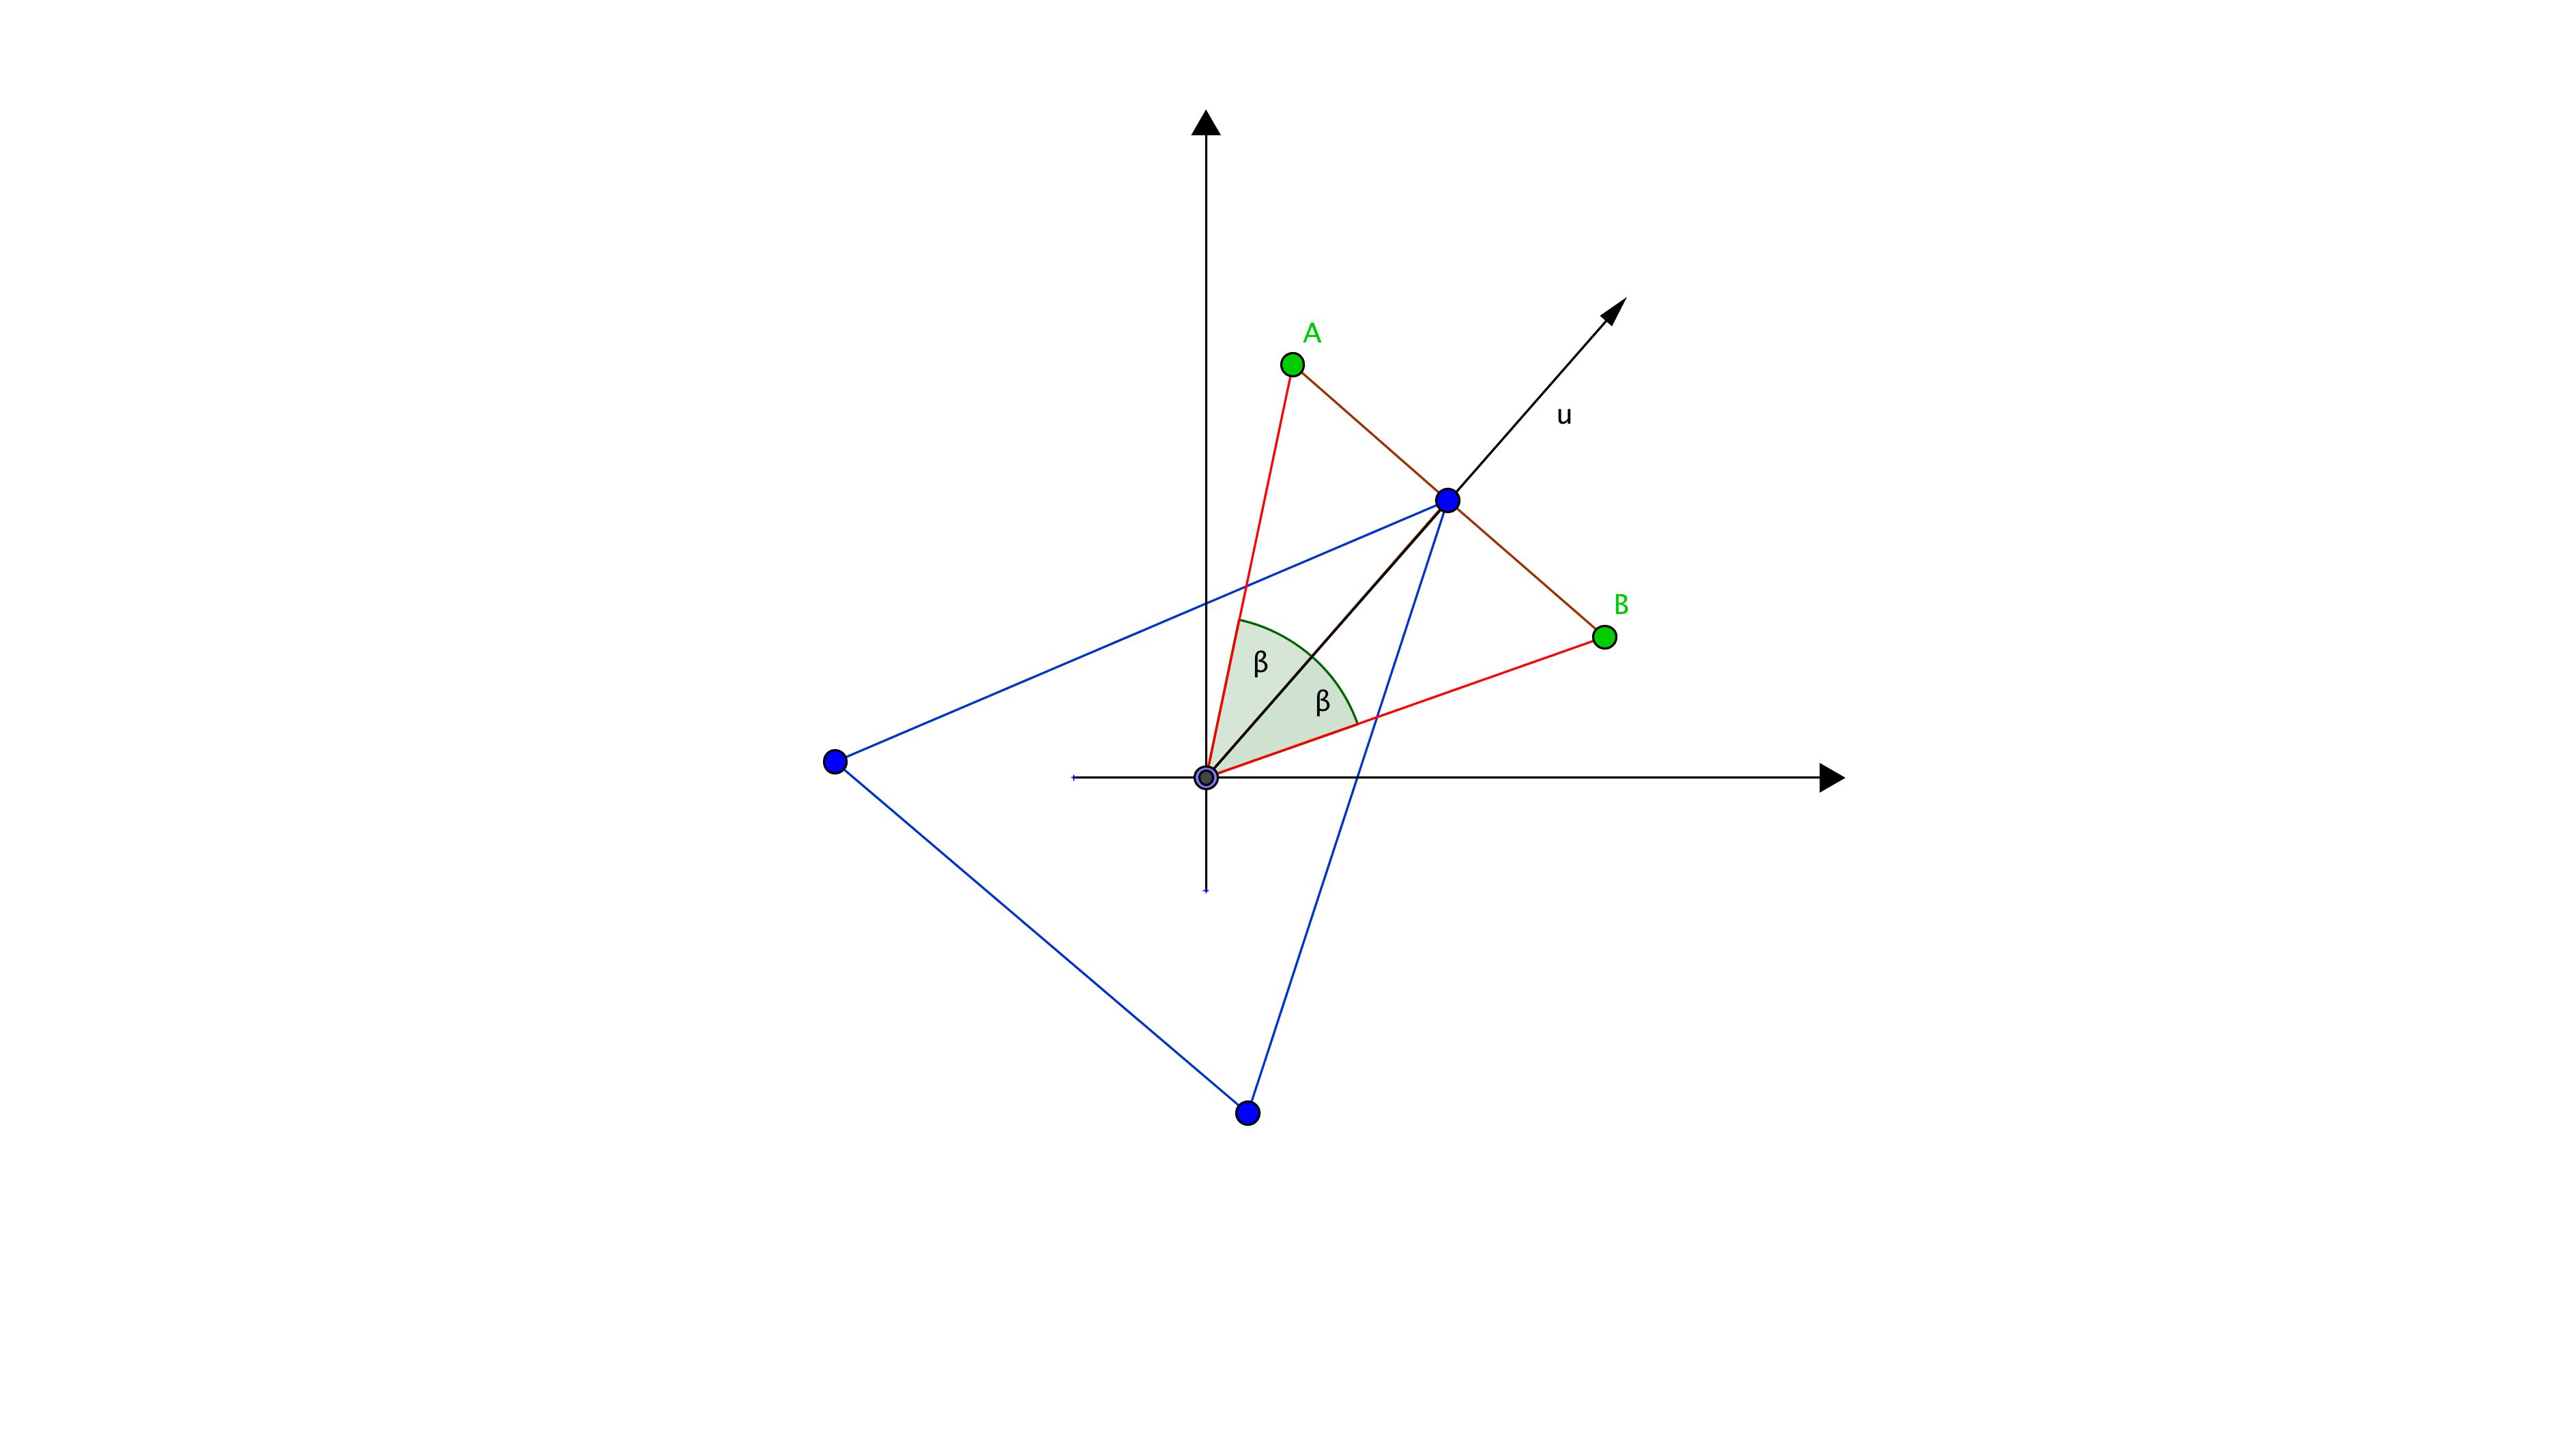
\includegraphics[scale=1]{images/lichtsensorgrafik.png} 
\caption{Die Abstraktion des Roboters zur Berechnung der Sensorpositionen}
\label{fig:roboter_abstrakt}
\end{figure}

Die Klasse \texttt{Roboter} enthält die Methoden zur Abfrage der Positionen der Sensoren im Bezug auf die x- und y-Achse: \texttt{gib\-X\-Licht\-Rechts()}, \texttt{gib\-Y\-Licht\-Rechts()}, \texttt{gib\-X\-Licht\-Links()} und \texttt{gibYLichtsLinks()}. Diese werden benötigt, um das Auslesen des Farbwerts des Pixels unter dem jeweiligen Sensor zu ermöglichen. Die eigentliche Abfrage des Helligkeitswertes passiert jedoch am Parcours-Objekt. In der zugehörigen Klasse steht die Methode \texttt{gibLichtmittelwert(int x, int y)} zur Verfügung, die auf das Bilddaten-Array zugreift. Da die realen Sensoren auch nicht nur einen einzelnen Punkt auf dem Boden, sondern einen Bereich abtasten, berechnet die Methode den Mittelwert aus neun Pixeln um die Position des Lichtsensors. Hierzu wird in der Methode \texttt{gib\-Hellig\-keits\-wert(int x, int y)} der Helligkeitswert jedes einzelnen der neun Pixel aus dem Bilddaten-Array abgefragt und der Mittelwert gebildet. Die Sensoren, die dann mit \texttt{gib\-Licht\-mittel\-wert(int x, int y)} die Helligkeit des ausgewählten Bereichs abfragen, bekommen das genormte Ergebnis (der Wert 0 entspricht schwarz, 100 entspricht weiß) des Mittelwerts ausgegeben.

Da sich die Farbsensoren in der Realität ähnlich verhalten wie die Lichtsensoren, ist die Implementation der Farbsensoren im Simulator code-identisch. Daher wird in dieser Ausarbeitung auf eine explizite Beschreibung verzichtet.

\subsubsection{Ultraschall- und Berührungssensor}
Der Berührungssensor, oder wie von leJOS TouchSensor genannt, ist im Simulator an der vordersten Spitze des Roboter-Objekts platziert. Da Hindernisse im Simulator schwerlich als mehrdimensionale Objekte dargestellt werden können, wird in diesem Prototyp zunächst mit einer Farbunterscheidung gearbeitet. Dies funktioniert wiederum über den Helligkeitswert der Pixel, die sich gerade unter der Spitze des Roboter-Objekts befindet. Die Position des Sonsors ergibt sich dabei in Anhängigkeit von der Größe des Roboters und seiner Ausrichtung. Sei $B$ die Breite des Roboters und $\alpha$ der Wert aus der Variablen \texttt{{\_}ausrichtung} des Roboters. Weiter entspreche $xPos$ der x-Position und $yPos$ der y-Position des Roboters. Dann folgt für die Koordinaten $\left( x \vert y \right)$ des Berührungssensors
\begin{align*}
dx & = \left( \sin \alpha \right) \cdot \left( \frac{B}{2} \right)\\
dy & = \left( \cos \alpha \right) \cdot \left( \frac{B}{2} \right)\\
 x & = xPos + dx\\
 y & = yPos - dy.
\end{align*}

Für die Implementation des Ultraschallsensors wird eine Implementation des Hindernisses als Objekt auf dem Parcours benötigt. Dies ist für die Implementation eine ersten Prototypen des Simulators nicht essentiell, da die für SuS relevanten Aufgaben auch mit einem Berührungssensor gelöst werden können. Daher verzichtet dieser Prototyp zunächst auf die Implementation eines Ultraschallsensors.

\subsubsection{Sensorports}
Jeder der eben genannten Sensoren ist an einen so genannten Sensorport angeschlossen. Die Klasse \texttt{SensorPort} enthält Felder, die die einzelnen Ports darstellen. Ein Exemplar einer Sensoren-Klasse wird bei der Initialisierung stets an einen Sensorport gekoppelt. 

\begin{figure}[htpb]
\centering
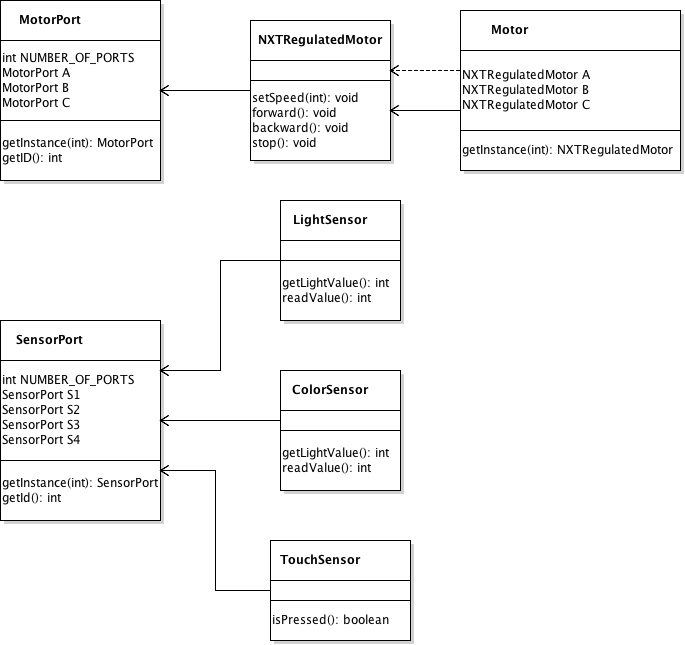
\includegraphics[scale=0.65]{images/uml_api_essenz.png}
\caption{UML-Diagramm der wichtigsten von leJOS NXJ vorgegebenen Klassen}
\label{fig:api_uml}
\end{figure}

\par \singlespacing
\subsection{Die Klassen des \texttt{sim}-Pakets}
\onehalfspacing
Nun zu einer Beschreibung der Struktur der Klassen, die für die Simulation zuständig sind. Hierzu gehört die grafische Repräsentation des Parcours, des Roboters, der Auswahldialog für den Parcours, sowie die Leinwand, auf der der simulierte Roboter fahren soll. Eine Gesamtübersicht der wichtigsten Klassen ist in \ref{fig:simulator_uml} abgebildet.

\subsubsection{Simulator}

Um die Simulationsumgebung aufzurufen, erzeugt man ein Exemplar der Klasse \texttt{Si\-mu\-la\-tor}. Der Konstruktor dieser Klasse ist so konzipiert, dass zunächst ein Parcours erzeugt und in diesem Zusammenhang eine Bilddatei mit dem gewünschten Parcours ausgewählt wird.\\
Als nächstes wird der Roboter über den Konstruktoraufruf \texttt{Roboter(335, 500)} auf den ausgewählten Parcours projiziert.\\
Die Klasse \texttt{Simulator} ist nicht nur für die Erzeugung der einzelnen Elemente der Simulationsumgebung zuständig, sondern auch für die Verwaltung des Prozessablaufs. Hierzu wird mit dem Aufrufen eines Simulators ein sogenannter \emph{Thread} erzeugt. Im Rumpf des Threads sind wiederum zwei Anweisungen innerhalb einer Endlosschleife zu finden. Zum einen der Befehl \emph{{\_}roboter.update();}, der dafür sorgt, dass der Status des Roboter-Objekts aktualisiert wird, zum anderen eine Verzögerung, ein \emph{Delay}, wodurch die Anweisungen in der Schleife alle Millisekunde neu durchlaufen werden. 


\subsubsection{Bildeinleser}
Die Klasse \texttt{BildEinleser} besitzt keinen Konstruktor, da diese nur als Hilfsklasse bestimmte Methoden zur Verfügung stellen muss. Durch den Aufruf der Methode\\
\texttt{liesBilddaten()} eines Bildeinlesers wird ein JFileChooser erzeugt, mithilfe dessen der Benutzer eine Bilddatei auswählen kann, auf der der Roboter simuliert werden soll. Danach wird das Bild so umgewandelt, dass ein Array aus Bildpunkten entsteht. Dies ist hilfreich für die spätere Arbeit mit Bewegungen und dem Einsatz von Sensoren auf dem Parcours, da auf jeden Datenpunkt des Parcours per Abruf der zugehörigen Array-Zelle zugegriffen werden kann.
%In dem dieser Arbeit vorangegangenen Studium wurde bereits mit Projekten gearbeitet, in denen Bilddateien eingelesen und benutzt wurden, daher wurde diese Klasse aus einem alten Projekt importiert.\\

\subsubsection{Parcours}
Der Parcours ist die Schnittstelle zwischen Simulator und den Klassen des \texttt{nxt-}Pakets. Sie ist unter anderem dafür zuständig, durch den Aufruf von \texttt{liesBilddaten()} am BildEinleser den Dialog für die Auswahl der Parcours-Grafikdatei zu erzeugen und die Bilddaten an die an dieser Stelle erzeugten Leinwand zu übergeben. Hierfür sind die implementierten Methoden \texttt{aktualisiere\-Bildgroes\-se(short[][] bild\-daten)}, \texttt{er\-zeu\-ge\-Lein\-wand()} und \texttt{zeichneBild()} zuständig. Insbesondere letztere übergibt die Bildpunkte in Form eines short-Arrays an die Leinwand.

Des Weiteren befindet sich in dieser Klasse die Implementation der Abfrage der Helligkeitswerte des Parcours, auf dem sich der Roboter befindet. Diese wurde mithilfe der beiden Methoden \texttt{gib\-Hellig\-keits\-wert(int x, int y)} und \texttt{gib\-Licht\-mittel\-wert(int x, int y)} realisiert. Die genauere Beschreibung der Funktionalität dieser Methoden ist im vorangegangenen Abschnitt über die Licht- und Farbsensoren zu finden.

\subsubsection{Leinwand}
Wie eben beschrieben, wird die Leinwand von dem Parcours erzeugt. Die Klasse Leinwand sorgt nun dafür, dass die als Array übergebenen Bildpunkte in einem JFrame, also vereinfacht einem neuen Fenster, angezeigt werden. \\
Des weiteren bietet die Leinwand eine Methode \texttt{warte()} an, die dafür genutzt wird, dass sich die Objekte auf der Leinwand tatsächlich animiert über den Hintergrund bewegen. Dies geschieht über den Aufruf \texttt{Thread.sleep(millisekunden)}, der dafür sorgt, dass der Prozess, der sich um das Zeichnen des Roboters kümmert, einige Millisekunden verzögert ausgeführt wird.

\subsubsection{Roboter}
Nun zum Kernstück der Simulationsumgebung, der Klasse \texttt{Roboter}. Diese enthält alle relevanten Informationen des Roboter-Objekts, wie die Position, die Ausrichtung, die Geschwindigkeit -- in Form von Variablen \texttt{{\_}xPos}, \texttt{{\_}yPos}, \texttt{{\_}aus\-rich\-tung},  \texttt{{\_}ge\-schwin\-dig\-keit} -- und das Aussehen. 

Sobald ein neuer Roboter erzeugt wird (\texttt{Roboter(int x, int y)}) wird das Bild des Roboters, welches zur Zeit noch ein einfaches Dreieck ist, eingelesen, auf die Leinwand gezeichnet und auf die übergebene Position gesetzt. Hierbei anzumerken ist, dass die Bilddatei einen imaginären Rahmen besitzt, so dass zwei Feldvariablen zur Positionskorrektur existieren, die für das Zeichnen auf der Leinwand benutzt werden. So ist sichergestellt, dass der Roboter auch tatsächlich an der übergebenen Position gezeichnet wird. Beim Konstruktoraufruf übergibt der Benutzer demnach den Mittelpunkt des Roboters.

Weiterer Bestandteil der Klasse ist die Methode \texttt{update()}. Diese ist dafür zuständig, dass der Roboter auf der Leinwand Bewegungen ausführen kann. Dies geschieht zunächst über die Veränderung der Ausrichtung des Roboters, wodurch natürlich eine Rotation der optischen Repräsentation des Roboters, also des Bildes, nötig ist. Die Methode \texttt{rotate(double Degrees)} erstellt in diesem Zusammenhang eine Kopie der ursprünglichen Robotergrafik, dreht diese um den angegebenen Winkel und ersetzt die bisher bestehende Grafik durch die gedrehte Kopie. Dieses Verfahren sorgt dafür, dass keine Pixelfehler und optischen Verwischungen an der Robotergrafik auf dem Parcours entstehen, da für jede Veränderung eine neue Kopie der Originalgrafik verwendet wird.

Abschließend wird nun der Roboter mithilfe der Methoden \texttt{setzePosition(int x, int y) und \texttt{zeichnen(int x, int y)}} auf der neuen Position auf dem Parcours gezeichnet. In Anlehnung an die leJOS API funktioniert dies über die Veränderung des Winkels und der Geschwindigkeit. Dies ist damit zu begründen, dass von den SuS nur die einzelnen Motoren angesteuert werden können, was dazu führt, dass jeweils nur durch eine Veränderung der Geschwindigkeit eines Motors das Fahren von Kurven möglich ist. Die Berechnung der neuen Position findet dabei wie folgt statt:

Die Feldvariable \texttt{{\_}win\-kel\-Ver\-än\-derung} bekommt durch den Aufruf der Methode \texttt{aen\-de\-re\-Be\-we\-gung(double win\-kel, double ge\-schwin\-dig\-keit)} in der Klasse NXTRegulatedMotor einen neuen Wert zugewiesen. Da dieser im Roboter-Objekt gespeichert ist, können wir direkt darauf zugreifen. Der in der Variablen \texttt{{\_}win\-kel\-Ver\-än\-derung} gespeicherte Wert wird nun zunächst auf die Feldvariable \texttt{{\_}ausrichtung} aufaddiert. Sei nun $\alpha$ der Wert der Variablen \texttt{{\_}ausrichtung} und $v$ die in der Variable \texttt{{\_}ge\-schwin\-dig\-keit} gespeicherte Geschwindigkeit. Des Weiteren entspreche $xPos$ dem Wert von \texttt{{\_}xPos}, sowie $yPos$ dem Wert von \texttt{{\_}yPos}. Dann folgt
\begin{align*}
dx & = \left( \sin \alpha \right) \cdot v\\
dy & = \left( \cos \alpha \right) \cdot v\\
x & = xPos + dx\\
y & = yPos - dy
\end{align*}
und die Zielkoordinaten des Roboters lauten $\left( x \vert y \right)$.

Abschließend werden der Roboter und seine Position durch den Aufruf \texttt{zeichnen(int x, int y)} an die Leinwand übergeben, die dafür sorgt, dass das neue Gesamtbild im Fenster angezeigt wird.\\
Im Zusammenspiel mit dem Thread, der in der Klasse Simulator erzeugt wird, führt der regelmäßige Aufruf der Methode \texttt{update()} zu der Bewegungsanimation des Roboters auf der Leinwand.


Des Weiteren enthält die Klasse \texttt{Roboter} eine Vielzahl von sondierenden Methoden, die die Positionskoordinaten des Roboters, sowie der Lichtsensoren und des Berührungssensors zurückgeben. Da bei der Implementation jeweils mit der Höhe und Breite, die durch weitere sondierende Methoden (\texttt{getHeight()} und \texttt{getWidth()}) an der Robotergrafik direkt ausgelesen werden können, gearbeitet wurde, besteht die Möglichkeit, relativ flexibel die Bilddatei des Roboters auszuwechseln (vgl. \textbf{\ref{sec:erweiterbarkeit}}).

\begin{figure}[htbp]
\centering
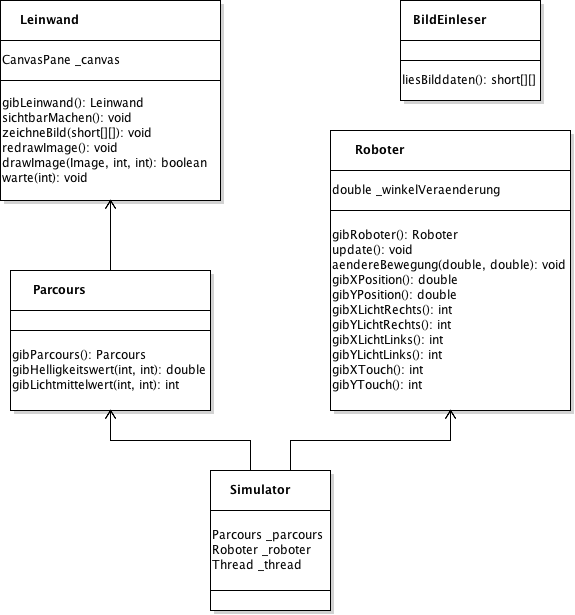
\includegraphics[scale=0.7]{images/uml_simulator_essenz.png}
\caption{UML-Diagramm der essentiellen Klassen für die Simulationsumgebung}
\label{fig:simulator_uml}
\end{figure}


\newpage
\chapter{Fazit und Ausblick}

\onehalfspacing

In dieser Masterarbeit wurde der Protoyp einer Java-Simulationsumgebung für \textsc{LEGO Mindstorms} NXT Roboter entwickelt. Das Ergebnis dieser Entwicklung ist die Möglichkeit, SuS ein Werkzeug zur Überprüfung ihres Quelltextes zur Steuerung des Roboters an die Hand
zu geben. Dieser Prototyp der Simulationsumgebung umfasst alle für die
Programmierung erster Software mit NXT Robotern essentiellen Klassen und deren Methoden und stellt eine Testumgebung für Sensoren und Motorbewegungen zur Verfügung.


\section{Umsetzung der Anforderungen}

Die Simulationsumgebung bietet den SuS die Möglichkeit, mit der von ihnen kennengelernten Sytax (auf Basis der leJOS NXJ API) ihre individuellen Lösungen direkt am Computer auszuprobieren. Hierbei müssen sie sich nicht mit einer neuen, zusätzlichen Benutzeroberfläche vertraut machen, sondern einfach nur zwei zusätzliche Anweisungen im Quellcode einfügen. Die Steuerung des NXT Roboters und des Roboters in der Simulation ist damit also nahezu code-identisch.

Bezüglich der realitätstreue der Parcours lässt sich zunächst sagen, dass die beispielhaft im Projekt mit enthaltenen Parcours Ausschnitte eines realen Parcours sein könnten. Dies stellt sicher, dass die SuS ihre Roboter in Testumgebungen fahren lassen können, die einen Bezug zu den Realbedingungen haben.

Außerdem kann jede Lehrkraft mithilfe eines Grafikprogramms weitere Parcours der Größe 740 x 640 Pixel entwerfen und den SuS zur Verfügung stellen. Es muss lediglich darauf geachtet werden, dass der Startpunkt der Roboters am Punkt (335 | 450) liegt und ggf. angepasst werden muss. Auch diese Informationen können in der Kurzanleitung nachgelesen werden. Auch dies gehörte zu den an die Simulationssoftware gestellten Anforderungen.

Zusätzlich zu den Kommentaren im Code, der den Lehrkräften zur Verfügung gestellt wird, ist im Anhang noch eine Kurzanleitung zu finden, die durch die Einbindung der Klassenbibliothek des Simulators in BlueJ führt, sowie Hinweise zur Benutzung enthält. Hierdurch kann ein leichtes Einarbeiten der Lehrkräfte in den Umgang mit der Simulationsumgebung gewährleistet werden. 

Die in \textbf{\ref{chap:anforderungen}} beschriebenen Anforderungen hinsichtlich der Schüler, Lehrer sowie der Erweiterbarkeit konnten demnach in einem guten Maße umgesetzt werden.

\section{Verbesserungen und Erweiterungen}

Da die entwickelte Simulationsumgebung bisher nur ein Prototyp ist, sollte sie folglich als nächstes in der Praxis getestet werden. Hierzu kann sie verschiedenen Lehrkräften zur Verfügung gestellt werden, die dann in unterschiedlichen Jahrgangsstufen damit arbeiten können. Dieser Schritt bewirkt, dass das Verhalten der Sensoren verfeinert und etwaige Fehler, die erst beim Testen mit von SuS geschriebenem Code auftreten, im Code lokalisiert und behoben werden können.\\
Damit einher geht auch der Umstand, dass das geforderte Verhalten der Sensoren bisher nur in einem beschränkten Maße getestet wurde. Dies bedeutet, dass eine hinreichend gute Approximation des Verhaltens der Sensoren beim Testen mit einem Mustercode erreicht wurde, dieser Mustercode aber nicht unbedingt den Realbedingungen entspricht. 

Des weiteren kann die Roboter-Grafik im Simulator, die bisher erst einmal zu Testzwecken aus einem Dreieck besteht, durch eine beliebige andere Grafik ausgetauscht werden, um den SuS das Gefühl, dass "`ihr"' Roboter im Simulator gerade die ersten Bewegungen vollführt, zu vermitteln.

Eine weitere Möglichkeit wäre auch, eine ähnlich wie bei \emph{Greenfoot} aufgebaute Steuerung der Simulation anbieten. Konkret würde dies bedeuten, dass der JFrame, in dem der Parcours angezeigt wird, um einen Bereich mit Buttons erweitert würde. Diese wären dann in der Lage, die Simulation zu starten, pausieren und anzuhalten.

Etwas umfassender, dafür aber eine schönere Integration in BlueJ mit sich bringend, wäre noch das Schreiben einer eigenen BlueJ Extension. Hierdurch würde die Möglichkeit entstehen, den Simulator gegebenenfalls direkt am Kontextmenü aufzurufen.

\newpage
\begin{thebibliography}{ABCD}

\renewcommand{\refname}{\normalsize Literaturverzeichnis}

\bibitem[Abe01]{abend:01}
Michael Abend. "'Robotik und Sensorik. Darstellungsschwerpunkt: Selbständige Entwicklung "`unscharfer"' Algorithmen zur räumlichen Orientierung (unter Verwendung des LEGO-Mindstorms-Systems)", \emph{Schriftliche Prüfungsarbeit zur zweiten Staatsprüfung für das Amt des Studienrats}, Berlin, 2001

\bibitem[Her12]{hertzberg:12}
Joachim Hertzberg, Kai Lingemann, Andreas Nüchter. \emph{Mobile Roboter. Eine Einführung aus Sicht der Informatik}, Springer-Verlag Berlin Heidelberg, 2012

\bibitem[Hub07]{hubwieser:07}
Peter Hubwieser. \emph{Didaktik der Informatik}, 3. Auflage, Springer-Verlag Berlin Heidelberg, 2007

\bibitem[Lego]{lego}
o.V. URL: \url{http://www.lego.com/en-us/mindstorms/history}, Abgerufen am 06.11.2015, LEGO, 2015

\bibitem[leJOS]{lejos}
o.V. URL: \url{http://www.lejos.org/nxj.php}, Abgerufen am 14.12.2015, leJOS Java for Lego Mindstorms, 2015

\bibitem[Nie99]{nievergelt:99}
Jürg Nievergelt. \emph{"Roboter programmieren" - ein Kinderspiel. Bewegt sich auch etwas in der Allgemeinbildung?}, Informatik-Spektrum 22:5, S. 364--375, 1999

\bibitem[Rol14]{rolling:14}
Mark Rollins. \emph{Beginning LEGO MINDSTORMS EV3}, Apress, Berkeley, CA, 2014

\bibitem[Sch04]{schreiber:04}
Rafael Schreiber. "Der Einsatz von LEGO-Mindstorms im Informatikunterricht der 11. Klasse der Leonard-Bernstein-Oberschule. Sicherung und Transfer grundlegender algorithmischer Strukturen in NQC.", \emph{Schriftliche Prüfungsarbeit im Rahmen der zweiten Staatsprüfung für das Amt des Studienrats}, Berlin, 2004

\bibitem[Sto01]{stolt:01}
Matthias Stolt. "Roboter im Informatikunterricht", 2001

\bibitem[Wag05]{wagner:05}
Oliver Wagner. "LEGO Roboter im Informatikunterricht. Eine Untersuchung zum Einsatz des LEGO-Mindstorms-Systems zur Steigerung des Kooperationsvermögens im Informatikunterricht eines Grundkurses (12. Jahrgang, 2. Lernjahr) der Otto-Nagel-Oberschule (Gymnasium)", \emph{Schriftliche Prüfungsarbeit im Rahmen der zweiten Staatsprüfung für das Amt des Studienrats}, Berlin, 2005

\end{thebibliography}
\newpage
\thispagestyle{empty}
\vspace*{\fill}
"Hiermit versichere ich, dass ich die Arbeit selbstständig verfasst und keine anderen als die angegebenen Hilfsmittel – insbesondere keine im Quellenverzeichnis nicht benannten Internet-Quellen – benutzt habe, die Arbeit vorher nicht in einem anderen Prüfungsverfahren eingereicht habe und die eingereichte schriftliche Fassung der auf dem elektronischen Speichermedium entspricht."\\

Hamburg, \today \hspace*{\fill} \dots \dots \dots \dots \dots \dots \dots\\
\hspace*{\fill} Pamina Maria Berg $\,$
\end{document}